%! Suppress = Unicode
%! Author = gsxab
%! Date = 2019/12/11

% Preamble
\documentclass[twocolumn,hidelinks,a4paper,10pt]{ctexart}

% Packages
% math
\usepackage{amsmath}
\usepackage{amsfonts}
\usepackage{amssymb}
\usepackage{amsopn}
\usepackage{amsthm}
\usepackage{bm}
% calculation
\usepackage{calc}
\usepackage{xstring}
% color
\usepackage[svgnames]{xcolor}
%% bib
%\usepackage{biblatex}
% font
%\usepackage{embrac}
\usepackage{enumitem}
\usepackage{geometry}
% footnote
\usepackage{pfnote}
% table
\usepackage{tabularx}
\usepackage{longtable}
\usepackage{booktabs}
\usepackage{makecell}
\usepackage{rotating}
\usepackage{multirow}
% illustration
\usepackage{graphicx}
\usepackage{tikz}
\usepackage{import}
\usepackage{xifthen}
\usepackage{pdfpages}
\usepackage{transparent}
\usepackage{subcaption}
\usepackage{lscape}
\usepackage{float}
% index
\usepackage[noautomatic]{imakeidx}
% bookmark
\usepackage[bookmarksnumbered=true]{hyperref}

% 偏右,左侧用于装订。
\geometry{
    left=27mm,
    right=6.3mm,
    top=12.7mm,
    bottom=12.7mm,
    headheight=12.7cm,
    headsep=4mm,
%    footskip=12mm,
    heightrounded,
}

\setCJKmainfont[BoldFont={SimHei}, ItalicFont={KaiTi}]{SimSun}
\setCJKsansfont{SimHei}
\setCJKmonofont{FangSong}

\setCJKfamilyfont{zhsong}{SimSun}
\setCJKfamilyfont{zhhei}{SimHei}
\setCJKfamilyfont{zhkai}{KaiTi}
\setCJKfamilyfont{zhfs}{FangSong}

\setmainfont[Mapping=tex-text]{Times New Roman}
\setsansfont[Mapping=tex-text]{Arial}
\setmonofont[Mapping=tex-text]{Consolas}

\theoremstyle{plain}
%\theoremstyle{definition}
\newtheorem{theorem}{定理}[section]
\newtheorem{proposition}[theorem]{命题}
\newtheorem{lemma}[theorem]{引理}
\newtheorem{corollary}[theorem]{推论}
\newtheorem{definition}[theorem]{定义}
\newtheorem{property}[theorem]{性质}
\newtheorem{examples}{举例}[section]
\newtheorem{abstraction}{抽象}[section]
\renewcommand*{\proofname}{证明}

\DeclareMathOperator{\card}{card}
\DeclareMathOperator{\DiagMatrix}{diag}
\DeclareMathOperator{\RankOf}{r}
\DeclareMathOperator{\TraceOf}{tr}
\DeclareMathOperator{\ud}{d} %用\ud 作为微分算子“d”
\newcommand{\transpose}{^\mathrm{T}}

\newcommand{\oldemptyset}{\emptyset}
\renewcommand{\emptyset}{\varnothing}

\newcommand{\VectorBase}[4]{{#1}_1#3\linebreak[1]{#1}_2#3\linebreak[1]#4#3\linebreak[1]{#1}_{#2}}
\newcommand{\VectorRBase}[5]{{#1}_{#3 1}#4\linebreak[1]{#1}_{#3 2}#4\linebreak[1]#5#4\linebreak[1]{#1}_{#3 #2}}
\newcommand{\VectorLBase}[5]{{#1}_{1#3}#4\linebreak[1]{#1}_{2#3}#4\linebreak[1]#5#4\linebreak[1]{#1}_{#2#3}}

\newcommand{\VectorComma}[2]{\VectorBase{#1}{#2}{,}{\dots}}
\newcommand{\VectorRComma}[3]{\VectorRBase{#1}{#2}{#3}{,}{\dots}}
\newcommand{\VectorLComma}[3]{\VectorLBase{#1}{#2}{#3}{,}{\dots}}
\newcommand{\Vector}[2]{\VectorBase{#1}{#2}{&}{\dots}}
\newcommand{\VectorR}[3]{\VectorRBase{#1}{#2}{#3}{&}{\dots}}
\newcommand{\VectorL}[3]{\VectorLBase{#1}{#2}{#3}{&}{\dots}}
\newcommand{\VectorNewLine}[2]{\VectorBase{#1}{#2}{\\}{\vdots}}
\newcommand{\VectorRNewLine}[3]{\VectorRBase{#1}{#2}{#3}{\\}{\vdots}}
\newcommand{\VectorLNewLine}[3]{\VectorLBase{#1}{#2}{#3}{\\}{\vdots}}

\newcommand{\Matrix}[1]{\begin{bmatrix}
                            #1
\end{bmatrix}}

\newcommand{\ExpandVectorComma}[2][n]{\begin{bmatrix}
                                          \VectorComma{#2}{#1}
\end{bmatrix}}
\newcommand{\ExpandVectorTab}[2][n]{\begin{bmatrix}
                                        \Vector{#2}{#1}
\end{bmatrix}}
\newcommand{\ExpandVectorNewLine}[2][n]{\begin{bmatrix}
                                            \VectorNewLine{#2}{#1}
\end{bmatrix}}
\newcommand{\ExpandMatrix}[2][m/n]{
\StrCut{#1}{/}\tmp\tmptmp
\begin{bmatrix}
    \VectorR{#2}{\tmptmp}{1}\\
    \VectorR{#2}{\tmptmp}{2}\\
    \vdots&\vdots&\ddots&\vdots\\
    \VectorR{#2}{\tmptmp}{\tmp}
\end{bmatrix}
}
\newcommand{\Transpose}{^\mathrm{T}}
\newcommand{\Hermitian}{^\mathrm{H}}

\newcommand{\textkw}[1]{\textsf{\textup{#1}}}
\newcommand{\indexedword}[1]{#1\index{#1}}
\newcommand{\indexed}[1]{\foreachdo{\indexedword}{#1}}
\newcommand{\indexedpair}[2]{\indexed{#1}(\indexed{#2})}
\newcommand{\keyword}[1]{\textkw{\indexed{#1}}}
\newcommand{\keywordpair}[2]{\textkw{\indexedpair{#1}{#2}}}

\newcommand{\foreachdo}[2]{%
\def\mystring{#2}%
\StrCut{\mystring}{/}\tmp\tmptmp%
#1{\tmp}%
\ifx\tmptmp\empty{}\else{/\foreachdo{#1}{\tmptmp}}\fi%
}

\renewcommand {\thetable} {\arabic{chapter}.\arabic{table}}
\renewcommand {\thefigure} {\arabic{chapter}.\arabic{figure}}
\renewcommand {\theequation} {\arabic{chapter}.\arabic{equation}}

\newcommand{\inputfig}[1]{
\import{./figures/}{#1.tikz}
}

\newcommand{\code}[1]{\texttt{#1}}
\setlist{noitemsep,topsep=0pt}
\setlength{\parskip}{.5em}
\hypersetup{final}

\title{南开大学软件学院硕士研究生专业数学基础课程复习笔记}
\author{gsxab}
\date{2019/12/11}

%\includeonly{tex/optimization-theory}

% Document
\begin{document}
%    \maketitle

    \part{矩阵论}
\section{$\lambda$矩阵与Jordan标准型}
\subsection{$\lambda$矩阵}

\begin{definition}[多项式矩阵~$\lambda$-矩阵]
    若$a_{ij}(\lambda),i=1,2,\dots,m,\linebreak[1]j=1,2,\dots,n$为$\lambda$的多项式,
    构成的矩阵$A(\lambda)$或记为$A$称为\textkw{多项式矩阵}或\textkw{$\lambda$-矩阵}。
\end{definition}

\begin{definition}[秩]
    $\lambda$-矩阵的秩定义为矩阵中最大的主子式并非全零的阶数。
    注意行列式为零指为多项式$0$,而不是能取到$0$。
\end{definition}

\begin{definition}[可逆~逆矩阵]
    对给定$n$阶方形$\lambda$-阵$A(\lambda)$,
    定义$A(\lambda)$可逆为$\exists B(\lambda),A(\lambda)B(\lambda)=B(\lambda)A(\lambda)=I$,
    称$B(\lambda)$为$A(\lambda)$的逆矩阵,记为$A^{-1}(\lambda)$。
\end{definition}

\begin{theorem}
    \[
        A^{-1}=\frac{1}{\det A(\lambda)} A^{*}(\lambda)
    \]
    其中右侧为行列式与伴随矩阵。
\end{theorem}

\begin{corollary}
    对方阵$A(\lambda)$,
    $A(\lambda)$可逆当且仅当$\det A(\lambda) \equiv c (c\neq 0)$。
\end{corollary}

\begin{definition}[初等变换~初等矩阵]
    $\lambda$-矩阵的初等变换:
    \begin{itemize}
        \item 交换两行
        \item 行乘$c$($c\neq 0$)
        \item 行乘以$\phi(\lambda)$加到另一行
    \end{itemize}
    单位矩阵施加以上操作得到的矩阵称为初等矩阵。
\end{definition}

\begin{theorem}
    初等矩阵均可逆。
\end{theorem}

\begin{corollary}
    初等矩阵的累积可逆,可逆矩阵可写作初等矩阵的积。
\end{corollary}

\begin{theorem}
    初等行变换等价于左侧乘以初等矩阵,初等列变换等价于右侧乘以初等矩阵。
\end{theorem}

\begin{definition}
    若$A(\lambda)$可经过有限次初等变换得到$B(\lambda)$,定义两$\lambda$-矩阵等价,记为$A(\lambda)\cong B(\lambda)$。
\end{definition}

\begin{corollary}
$A\cong B \Leftrightarrow \exists P(\lambda),Q(\lambda), B(\lambda) = P(\lambda) A(\lambda) Q(\lambda)$
\end{corollary}

\subsection{Smith标准型与不变因子、行列式因子}

\begin{definition}[Smith标准型~不变因子]
%    对任意$m\times n$ $\lambda$-矩阵$A(\lambda)$,
    对任意$n$阶$\lambda$-矩阵$A(\lambda)$,
    总是有对角阵$\DiagMatrix(d_1(\lambda),d_2(\lambda),\dots,\linebreak[1]d_r(\lambda),0,\dots,0)$与之等价。
    其中$d_i(\lambda)$都是首项系数为$1$的多项式,且$d_i|d_{i+1}$。
    称这个对角阵为$A(\lambda)$的\textkw{Smith标准型},其中$d_i(\lambda)$称为$A(\lambda)$的\textkw{不变因子}。
\end{definition}

\begin{definition}[行列式因子]
    对$A(\lambda)$,定义所有$k$阶子式的最大公因式$D_k(\lambda)$为$A(\lambda)$的$k$阶\textkw{行列式因子}。
    约定其首项系数为$1$。
\end{definition}

\begin{property}
    行列式因子具有以下性质:
    \begin{itemize}
        \item $D_i(\lambda)|D_{i+1}(\lambda)$
        \item $D_i=1\Rightarrow D_{i-1}=D_{i-2}=\dots=D_1=1$
        \item 存在$k$阶子式非零常数,则$D_k=1$
        \item 存在两个$k$阶子式无公因式,则$D_k=1$
        \item $D_k(\lambda)=a\det A(\lambda)$
    \end{itemize}
\end{property}

\begin{theorem}
    初等变换不改变行列式因子和秩。
\end{theorem}

\begin{theorem}
    $D_k(\lambda)=\prod\limits_{i=1}^{k} d_i(\lambda)$
\end{theorem}

\begin{corollary}
    \[
        A\cong B
        \Leftrightarrow \forall k, D_{Ak}(\lambda) = D_{Bk}(\lambda)
        \Leftrightarrow \forall i, d_{Ai}(\lambda) = d_{Bi}(\lambda)
    \]
\end{corollary}

\begin{theorem}
    Smith标准型唯一。
\end{theorem}

\begin{theorem}
    \[
        A(\lambda)\text{可逆}\Leftrightarrow A(\lambda)\cong I
    \]
\end{theorem}

\subsection{初等因子}

\begin{definition}
    按$d_r(\lambda)$的$s$个互异复根$\lambda_j$分解多项式为一次多项式之积,则由整除关系,
    $d_i=\prod_j (\lambda-\lambda_j)^{e_{ij}},i=1,2,\dots,r,j=1,2,\dots,s$,且$0\leq e_{1j}\leq e_{2j} \leq\dots\leq e_{rj}$。
    其中全部指数大于零的因子$(\lambda-\lambda_j)^{e_{ij}}$,允许重复,称为其\textkw{初等因子}。
\end{definition}

举例:
\[
    \begin{aligned}
        d_{1}(\lambda) &= 1 \\
        d_{2}(\lambda) &= \lambda(\lambda-1) \\
        d_{3}(\lambda) &= \lambda(\lambda-1)^{2}(\lambda+1)^{2} \\
        d_{4}(\lambda) &= \lambda^{2}(\lambda-1)^{3}(\lambda+1)^{3}(\lambda-2) \\
    \end{aligned}
\]
则$A(\lambda)$初等因子为$\lambda, \lambda, \lambda^{2}, \lambda-1, (\lambda-1)^{2},(\lambda-1)^{3},(\lambda+1)^{2},(\lambda+1)^{3},(\lambda-2)$

\begin{property}
    若不变因子相同,初等因子必然相同。若初等因子相同且秩相同,不变因子必然相同。
\end{property}
前者显然,后者是因为同一个根构成的$k$个因子一定分别是来自$d_r,d_{r-1},\dots,d_{r-k+1}$的因子。

\begin{corollary}
    矩阵等价当且仅当有相同的秩和初等因子。
\end{corollary}

\begin{theorem}
    分块对角矩阵的初等因子的全体为所有子矩阵的初等因子的全体。
\end{theorem}

\subsection{数字矩阵相似与$\lambda$矩阵等价}
\begin{theorem}
    数字矩阵$A,B$相似当且仅当$\lambda I-A,\lambda I-B$等价。
\end{theorem}

\begin{definition}
    对数字矩阵$A$,称$\lambda I - A$的不变因子、初等因子为$A$的不变因子、初等因子。
\end{definition}

考虑对数字矩阵$A$,$\lambda I-A$必然满秩,有
\begin{definition}
    对数字矩阵$A,B$,以下条件等价:
    \begin{itemize}
        \item 相似。
        \item 有相同初等因子。
        \item 有相同不变因子。
        \item 有相同行列式因子。
    \end{itemize}
\end{definition}

\subsection{Jordan标准型}

\subsubsection{求解等价的标准型}

\begin{theorem}
    对数字矩阵$A$,记初等因子为$\left(\lambda-a_{1}\right)^{n_{1}},\linebreak[1]\left(\lambda-a_{2}\right)^{n_{2}},\cdots,\left(\lambda-a_{s}\right)^{n_{s}}$,
    则$A\sim J$,其中$J$是Jordan矩阵$J=\DiagMatrix(J_1,J_2,\dots,J_s)$,且$J_i$是对角元为$a_i$的$n_i$阶Jordan块。
\end{theorem}

\begin{corollary}
    数字矩阵$A$可以对角化当且仅当初等因子都是一次式。
\end{corollary}

通过特征值和矩阵秩也可用于求解Jordan标准型。
每个特征值的代数重数(特征多项式根的重数)是特征值在对角线上出现的次数,
即对应Jordan块阶数和,
几何重数(对应不变子空间维数)是Jordan块数。
但是这个方法没办法区分Jordan块的划分,
如果存在同一特征值的2个2阶Jordan块和1个1阶1个3阶都会表现为代数重数4,几何重数2。
因此这一方法仅能用于低阶矩阵Jordan标准型的求解。

\begin{theorem}
    \[
        \begin{bmatrix}
            a & b\\
              & a
        \end{bmatrix}
        \sim
        \begin{bmatrix}
            a & 1 \\
              & a \\
        \end{bmatrix}
    \]
\end{theorem}

\subsubsection{求解相似变换矩阵}
关于
\[
    P^{-1}AP=J
\]
求解$P$。

\[
    AP=PJ
\]
按若尔当矩阵分块书写这一矩阵可得关于向量的方程组,
\[
    \left[A P_{1}, A P_{2}, \cdots, A P_{t}\right]=\left[P_{1} J_{1}, P_{2} J_{2}, \cdots, P_{t} J_{t}\right]
\]
在每一个$A P_i = P_i J_i$中,按列分块$P=[X_1,X_2,\dots,X_{n_i}]$有
\[
    \begin{split}
        A X_1 &= \lambda_i X_1 \\
        A X_2 &= X_1+ \lambda_i X_2\\
        A X_3 &= X_2+ \lambda_i X_3 \\
        &\dots \\
        A X_n &= X_{n_i-1}+\lambda_i X_{n_i}\\
    \end{split}
\]
$X_1$的选取需要保证$X_2$有解,依此类推,且需要解出线性无关的特征向量。

\section{内积空间、正规矩阵与Hermite阵}

\subsection{内积空间}

\subsubsection{内积空间}

\begin{definition}[内积空间]
    对给定$F=\mathbb{C}$上的向量空间$V$,
    定义一个$V\times V\to F, \alpha,\beta\mapsto (\alpha,\beta)$的运算$(\alpha,\beta)$,
    若这个运算满足:
    \begin{itemize}
        \item 共轭对称性$(\alpha,\beta)=\overline{(\beta,\alpha)}$
        \item 对$\alpha$线性$(\alpha_1+\alpha_2, \beta)=(\alpha_1,\beta)+(\alpha_2,\beta),(k\alpha,\beta)=k(\alpha,\beta)$
        \item 正定性$(\alpha,\alpha)\geq 0$,且$(\alpha,\alpha)=0\Leftrightarrow \alpha=\bm{0}$
    \end{itemize}
    称这个运算是一个\textkw{内积}运算。
    增添了内积结构的复向量空间称为\textkw{酉空间},实数域上为\textkw{欧几里得空间},统称内积空间。
\end{definition}

\begin{property}
    \begin{gather*}
        \left(\sum_{i=1}^{t} k_{i} \alpha_{i}, \beta\right) =\sum_{i=1}^{t} k_{i}\left(\alpha_{i}, \beta\right) \\
        \left(\alpha, \sum_{i=1}^{t} k_{i} \beta_{i}\right) =\sum_{i=1}^{t} \bar{k}_{i}\left(\alpha, \beta_{i}\right)
    \end{gather*}
\end{property}

\begin{definition}[度量矩阵]
    对$n$维酉空间$V$上的一组基$\{\alpha_i\}$,定义
    \[
        G=\Big((\alpha_i, \alpha_j)\Big)_{n\times n}
    \]
    为基底$\{\alpha_i\}$的度量矩阵。
\end{definition}

\begin{property}
    度量矩阵是Hermite阵。
\end{property}

已省略其他定义。
\begin{itemize}
    \item 内积
    \item 酉空间/欧氏空间
    \item 长度
    \item 夹角
    \item 单位化
    \item 正交向量组/正交基
    \item 标准正交向量组/标准正交基
    \item Schmidt正交化
\end{itemize}

\subsubsection{酉矩阵/正交矩阵}

\begin{definition}
    Hermite算子${}\Hermitian$定义为$A\Hermitian=\bar{A}\Transpose=\overline{A\Transpose}$,称为$A$的共轭转置矩阵。
    对方阵$A$,若$A=A\Hermitian$定义为Hermite阵,简称H-阵;若$A=-A\Hermitian$定义为反Hermite阵,简称反H-阵。
    对应实数域上的对称矩阵和反对称矩阵。
\end{definition}

\begin{definition}
    定义满足$U U\Hermitian=U\Hermitian U=I$的$n$阶方阵$U$为酉矩阵,记集合为$U\in U^{n\times n}$。
    实数域上为正交矩阵。
\end{definition}

\begin{theorem}
    Householder阵$H=I-2\alpha\alpha\Hermitian,|\alpha|=1$为酉矩阵。
\end{theorem}

\begin{property}
    若$A$为酉矩阵:
    \begin{itemize}
        \item $A^H=A^{-1}\in U^{n\times n}$
        \item $|\det A|=1$
        \item $AB,BA\in U^{n\times n}$
    \end{itemize}
\end{property}

\begin{theorem}
    给定矩阵,是酉矩阵当且仅当列向量标准正交。
\end{theorem}

\begin{definition}
    定义酉空间上保持内积不变的线性变换为酉变换。
    欧氏空间上保持内积不变的称为正交变换。
\end{definition}

\begin{property}
    酉变换保持向量的长度、夹角不变。
\end{property}

\begin{theorem}
    给定酉空间$V$和$V$上线性变换$\sigma$,以下等价:
    \begin{itemize}
        \item $\sigma$是酉变换
        \item $\forall \alpha\in V, \|\sigma(\alpha)\|=\|\alpha\|$
        \item 将$V$中的一组标准正交基变换为标准正交基
        \item $\sigma$在标准正交基下的表示为酉矩阵
    \end{itemize}
\end{theorem}

\begin{definition}[次酉矩阵]
    给定列满秩矩阵$U\in \mathbb{C}^{m\times r}_r$,若列向量标准正交,称为\textkw{次酉矩阵},记$U\in U^{m\times r}_r$。
\end{definition}

\begin{theorem}
    给定$U\in \mathbb{C}^{m\times n}$,$U$是次酉矩阵当且仅当$U\Hermitian U=I_r$。
\end{theorem}

\subsubsection{幂等矩阵}

\begin{definition}
    对方阵$A$,若$A^2=A$,称$A$幂等。
\end{definition}

\begin{property}
    给定幂等矩阵$A$,有:
    \begin{itemize}
        \item $A\Transpose,A\Hermitian,I-A$幂等
        \item $A(I-A)=(I-A)A=0$
        \item $\operatorname{N}(A)=\operatorname{R}(I-A)$
        \item $Ax=x\Leftrightarrow x\in R(A)$
        \item $\mathbb{C}^n=\operatorname{R}(A)\oplus \operatorname{N}(A)$
    \end{itemize}
\end{property}

\begin{theorem}
    $A\in \mathbb{C}^{n\times n}_r$,$A$幂等$\Leftrightarrow A\sim \DiagMatrix{(I_r,\bm{0}_{n-r})}$
\end{theorem}

\begin{corollary}
    $A$幂等$\Rightarrow \RankOf(A)=\TraceOf(A)$
\end{corollary}

\begin{theorem}
    方阵$A$,$A$幂等,当且仅当,存在次酉矩阵$U\in U^{n\times r}_r$,使得$A=U U\Hermitian$
\end{theorem}

\subsection{正规矩阵}

\subsubsection{Schur引理与Schur不等式}

\begin{theorem}[Schur引理]
    任意一个复方阵$A\in \mathbb{C}^{n\times n}$酉相似于一个上三角阵。
\end{theorem}
可使用数学归纳法,根据基的扩充定理和施密特正交化证明。

\begin{definition}
    给定$n$阶方阵$A$,有
    \[
        U\Hermitian AU= T=
        \begin{bmatrix}
            \lambda_1 & \cdots & *\\
            & \ddots & \vdots \\
            && \lambda_n \\
        \end{bmatrix}
    \]
    则有
    \[
        A=UTU\Hermitian
    \]
    称为$A$的Schur分解。
\end{definition}

\begin{theorem}[Schur不等式]
    对给定$n$阶方阵$A=\Big(a_{ij}\Big)_{n\times n}$,特征值为$\VectorComma{\lambda}{n}$,
    有
    \[
        \sum_i |\lambda_i|^2 \leq \sum_i \sum_j |a_{ij}|^2
    \]
\end{theorem}

\subsubsection{正规矩阵}

\begin{definition}[正规矩阵]
    对方阵$A$,若$AA\Hermitian=A\Hermitian A$,称为\textkw{正规矩阵}。
    实数域上称实正规矩阵。
\end{definition}

\begin{lemma}
    与正规矩阵酉相似的矩阵一定是正规矩阵。
\end{lemma}

\begin{lemma}
    同时是正规矩阵、三角形矩阵,则必然是对角矩阵。
\end{lemma}

\begin{theorem}
    正规矩阵的充要条件是酉相似于对角矩阵。
\end{theorem}

\begin{corollary}
    正规矩阵有n个线性无关特征向量,且对应不同特征值的特征向量互相正交。
\end{corollary}

\begin{theorem}
    对正规矩阵:
    \begin{itemize}
        \item 是Hermite矩阵,当且仅当,特征值全部落在实轴上。
        \item 是反Hermite矩阵,当且仅当,特征值全部落在虚轴上。
        \item 是酉矩阵,当且仅当,特征值全部落在单位圆上。
    \end{itemize}
\end{theorem}

\subsection{Hermite二次型}
\subsubsection{Hermite矩阵}

\begin{theorem}
    对Hermite矩阵$A$,有:
    \begin{itemize}
        \item $A\Hermitian A,AA\Hermitian$都是Hermite矩阵。
        \item $A+A\Hermitian$是Hermite矩阵,但$A-A\Hermitian$是反Hermite矩阵。
        \item $A^k$是Hermite矩阵,若可逆,$A^{-1}$也是Hermite矩阵。
        \item $\lambda\in \mathbb{R}$,则$\lambda A$是Hermite矩阵,$\lambda iA$是反Hermite矩阵。
    \end{itemize}
    对Hermite矩阵$A,B$,有:
    \begin{itemize}
        \item 实系数线性组合也是Hermite矩阵。
        \item 乘积$AB$是Hermite矩阵当且仅当可交换。
    \end{itemize}
\end{theorem}

\begin{theorem}
    对方阵$A\in\mathbb{C}^n$,以下三项等价:
    \begin{itemize}
        \item $A$是Hermite矩阵
        \item $\forall X\in \mathbb{C}^n$,$X^H A X$是实数
        \item $\forall B\in \mathbb{C}^{n\times n}$,$B^H A B$是Hermite矩阵
    \end{itemize}
\end{theorem}

\subsubsection{Hermite二次型}

\begin{definition}[Hermite二次型]
    $n$个复变量$\VectorComma{x}{n}$,二次齐次多项式
    \[
        f(\VectorComma{x}{n})=\sum_{i,j} a_{ij} \overline{x_i} x_j
    \]
    其中$a_{ij}=\overline{a_{ji}}$,
    则称为\textkw{Hermite二次型}。

    类似实数域上二次型的记号,
    记向量$X=(\VectorComma{x}{n})\Transpose$,矩阵$A=\Big(a_{ij}\Big)_{m\times n}$,
    则
    \[
        f(\VectorComma{x}{n}) = X\Hermitian A X
    \]
    其中矩阵$A$称为\textkw{Hermite二次型的的矩阵},是一个Hermite阵,
    $A$的秩为\textkw{Hermite二次型的秩}。
\end{definition}

可以对Hermite二次型进行可逆线性替换,即使用$X=CY$,其中$C$为可逆方阵,代替,得到
\[
    X\Hermitian A X = Y\Hermitian C\Hermitian A C Y = Y\Hermitian B Y
\]

\begin{definition}
    矩阵为对角矩阵的Hermite二次型
    \[
        f()=\lambda_1\overline{x_1}x_1+\lambda_2\overline{x_2}x_2+\dots+\lambda_n\overline{x_n}x_n
    \]
    称为二次型的标准型。
\end{definition}

\begin{theorem}
    对给定Hermite二次型,总是存在酉线性替换将其转化为标准型。
    存在举例:标准型的对角矩阵的对角线元素为原矩阵的特征值。
    这一线性替换的分解就是原矩阵的特征值分解。
    但线性替换是合同不是相似,不要求酉线性替换的情况下,变换结果对角矩阵不唯一。
\end{theorem}

\begin{definition}
    矩阵为对角矩阵,且对角线上元素具有前$s$个为$1$,然后$r-s$个元素为$-1$,其余$n-r$个为$0$的形式
    \[
        f()=\overline{x_1}x_1+\dots+\overline{x_s}x_s-\overline{x_{s+1}}x_{s+1}-\dots-\overline{x_r}x_r
    \]
    的二次型称为二次型的规范型。
\end{definition}

\begin{theorem}
    对给定Hermite二次型,总是存在唯一对应的规范型。
    矩阵的标准型总是有固定的正系数、负系数、零系数项(正负惯性指数),
    将其按这个顺序重排并将其绝对值平方根转换到两侧线性替换中,则得到规范型矩阵。
\end{theorem}

\subsubsection{正定Hermite二次型}

由Hermite矩阵的性质,对任意$X$都有$X\Hermitian AX$为实数,因此Hermite二次型结果总是实数。

\begin{definition}[正定~半正定]
    对Hermite矩阵$A$,
    若$\forall X\in \mathbb{C}^{n}\setminus\{\bm{0}\},X\Hermitian AX>0$,称$A$正定;
    若$\forall X\in \mathbb{C}^{n}, X\Hermitian AX \geq 0$,称$A$半正定。
\end{definition}

\begin{theorem}
    对给定Hermite二次型$f(X)=X\Hermitian AX$,以下各项等价:
    \begin{itemize}
        \item $f(X)$正定
        \item 对任意可逆$P$,$P\Hermitian AP$正定
        \item $A$的$n$个特征值均为正数(正惯性指数为$n$)
        \item 存在可逆$P$,$P\Hermitian AP=I$(规范型)
        \item 存在可逆$Q$,$A=Q\Hermitian Q$(上一条的推论)
        \item 存在正线上三角$R$,$A=R\Hermitian R$
    \end{itemize}
\end{theorem}

\begin{theorem}
    对给定Hermite二次型$f(X)=X\Hermitian AX$,以下各项等价:
    \begin{itemize}
        \item $f(X)$半正定
        \item 对任意可逆$P$,$P\Hermitian AP$半正定
        \item $A$的$n$个特征值均为非负实数(负惯性指数为$0$)
        \item 存在可逆$P$,$P\Hermitian AP=\DiagMatrix(I_r, \bm{0})$(规范型)
        \item 存在秩为$r$的$n$阶方阵$Q$,$A=Q\Hermitian Q$(上一条推论)
    \end{itemize}
\end{theorem}

\begin{theorem}
    $A$为正定(半正定)Hermite矩阵,则存在唯一的正定(半正定)$Q$,满足$A=Q^2$。
    记为$Q=A^{\frac{1}{2}}$。
\end{theorem}

\subsubsection{Hermite矩阵偶合同标准型}

\begin{theorem}
    对给定二次型$A,B$,若$B$正定,存在非退化线性替换$X=PY$同时满足:
    \begin{gather*}
        P\Hermitian AP = \sum_{i=1}^n \lambda_i \overline{y_i} y_i \\
        P\Hermitian BP = \sum_{i=1}^n \overline{y_i} y_i
    \end{gather*}
    其中$\lambda_i$是$|\lambda B-A|=0$的根,且均为实数。
\end{theorem}

先对角化$B$并化为规范型,即$P_1\Hermitian BP_1=I$,其中$P_1$可逆,
因此$P_1\Hermitian AP_1$也是正定矩阵,
然后酉相似对角化$P_1\Hermitian AP_1$,
得到$P_2\Hermitian P_1\Hermitian A P_1 P_2=\Lambda$,
其中$P_2$为酉矩阵。
此时有$P_2\Hermitian P_1\Hermitian B P_1 P_2 = P_2\Hermitian I P_2 = I$,
因此可逆矩阵$P=P_1 P_2$即为符合条件的方阵。

\begin{definition}
    对给定$n$阶Hermite矩阵$A,B$,其中$B$正定,则使方程
    \[
        AX=\lambda BX
    \]
    有非零解的$\lambda$的充要条件是
    \[
        |\lambda B-A|=0
    \]
    类比与特征方程、特征值与特征向量,
    称这个关于$\lambda$的方程为矩阵$A$相对于矩阵$B$的特征方程,
    根$\VectorComma{\lambda}{n}$为$A$相对于$B$的广义特征值,
    关于$\lambda=\lambda_i$时$X$的方程的解向量为对应$\lambda_i$的广义特征向量。
\end{definition}

\begin{property}
    给定Hermite矩阵$A,B$,其中$B$正定,则$A$相对于$B$,
    总是有$n$个广义特征值,且分别对应$n$个线性无关的广义特征向量。
    适当选取广义特征向量$\VectorComma{X}{n}$,
    可满足$X_i\Hermitian B X_j=\delta_{ij},X_i\Hermitian A X_j = \lambda_j\delta_{ij}$
\end{property}

\section{矩阵的分解}
\subsection{满秩分解}

\begin{definition}[满秩分解]
    对矩阵$A\in \mathbb{C}^{m\times n}_r$,
    $\exists B\in \mathbb{C}^{m\times r}_r, C\in \mathbb{C}^{r\times n}_r$,
    使得$A=BC$,称为矩阵的满秩分解。
\end{definition}

求解方法:
\begin{enumerate}
    \item 将矩阵$A$化为行最简形/rref得到$R$,获得主元位置。
    \item $A$中主元所在列构成$B$。
    \item $R$中主元所在行构成$C$。
\end{enumerate}

\begin{theorem}
    矩阵的满秩分解不唯一,若$A=BC=B_1 C_1$均为$A$的满秩分解,有:
    $\exists \theta\in \mathbb{C}^{n\times n}_n, B=B_1 \theta, C=\theta^{-1} C_1$,且
    具有不变量$C\Hermitian(C C\Hermitian)^{-1} (B\Hermitian B)^{-1} B\Hermitian$。
\end{theorem}

\subsection{正交三角分解}

\begin{definition}[正交三角分解]
    给定可逆方阵$A\in \mathbb{C}^{n\times n}_n$,存在唯一的酉矩阵$U$和正线上三角阵$R$使得$A=UR$;
    对于转置的情况,存在唯一的酉矩阵$U_1$和正线下三角阵$R_1$使得$A=R_1 U_1$
\end{definition}

\begin{theorem}
    给定矩阵$A\in \mathbb{C}^{m\times r}_r$,存在唯一的次酉矩阵$U\in U^{m\times r}$和$r$阶正线上三角矩阵$R$使得$A=UR$。
\end{theorem}

求法:
\begin{enumerate}
    \item 将$A$的列向量组施密特正交化得到$U$。
    \item $A=UR\Rightarrow R=U\Hermitian A$
\end{enumerate}

\begin{corollary}
    对给定矩阵$A\in \mathbb{C}^{m\times n}_r$,存在一个分解$A=U_1 R_1 L_2 U_2$,
    其中$U_1\in U^{m\times r},U_2\in U^{r\times n}$,且$R_1,L_2$为$r$阶上三角阵和下三角阵。
\end{corollary}

\subsection{奇异值分解}

\begin{lemma}
    对任意矩阵$A$,有$r(AA\Hermitian)=r(A\Hermitian A)=r(A)$
\end{lemma}

\begin{lemma}
    对任意矩阵$A$,有$AA\Hermitian$和$A\Hermitian A$都是半正定Hermite阵。
\end{lemma}

\begin{theorem}
    对任意矩阵$A\in \mathbb{C}^{m\times n}_r$,记
    $AA\Hermitian$的特征值从大到小排列为$\lambda_1\geq \lambda_2\geq \dots \geq \lambda_r > \lambda_{r+1}=\dots = \lambda_m = 0$,
    $A\Hermitian A$的特征值从大到小排列为$\mu_1\geq \mu_2\geq \dots \geq \mu_r > \mu_{r+1}=\dots = \mu_n = 0$,
    则有$\lambda_i = \mu_i >0, i=1,2,\dots,r$。
\end{theorem}

\begin{theorem}
    对正规矩阵$A$,$AA\Hermitian$和$A\Hermitian A$的特征值是$A$的特征值的模长平方。
\end{theorem}

\begin{definition}[奇异值]
    对矩阵$A\in \mathbb{C}^{m\times n}_r$,记$AA\Hermitian$的非零特征值从大到小排列为$\VectorComma{\lambda}{r}$,
    称$\sigma_i = \sqrt{\lambda_i} = \sqrt{\mu_i} > 0$为矩阵的正奇异值,简称奇异值。
\end{definition}

\begin{theorem}
    对矩阵$A\in \mathbb{C}^{m\times n}_r$,记奇异值为$\sigma_1\geq \sigma_2\geq \dots \sigma_r$,
    则存在$U\in U^{m\times m},V\in U^{n\times n}$,
    使得$U\Hermitian AV=\begin{bmatrix}\Delta & \bm{0} \\ \bm{0} & \bm{0} \end{bmatrix}$,
    其中$\Delta = \DiagMatrix(\VectorComma{\sigma}{r})$为奇异值由大到小排列构成的对角阵,
    填充$0$后的矩阵为$m\times n$矩阵。
\end{theorem}

\begin{definition}[奇异值分解]
    对矩阵$A$,定义$A=U\begin{bmatrix}\Delta & \bm{0} \\ \bm{0} & \bm{0} \end{bmatrix} V\Hermitian$为矩阵的奇异值分解式。
\end{definition}

考虑将$U,V$的前$r$列与后$m-r$和$n-r$列分块,则得到$A=U_1 \Delta V_1$,即:
\begin{corollary}
    对矩阵$A\in \mathbb{C}^{m\times n}_r$,记奇异值为$\sigma_1\geq \sigma_2\geq \dots \sigma_r$,
    存在次酉矩阵$U\in U^{m\times r},V\in U^{r\times n}$,使得$A = U \Sigma V\Hermitian$
\end{corollary}

求解方法:
\begin{enumerate}
    \item 计算$AA\Hermitian$(或$A\Hermitian A$)。
    \item 特征值分解$AA\Hermitian$(或$A\Hermitian A$),得到特征值$\VectorComma{\lambda}{r}$,以及对应标准正交特征向量组,分别构成对角矩阵$\Delta$和酉矩阵$U$(或$V$)。
    \item 将$U$分块,记对应非零特征值的前$r$列为$U_1$,对应特征值$0$的后$m-r$列为$U_2$。同样记$V$的前$r$列与后$n-r$列为$V_1,V_2$。
    \item $A=U_1\Delta V_1\Hermitian\Rightarrow U_1=A V_1\Delta^{-1} V_1, = A\Hermitian U_1\Delta^{-1}$。求出另一个矩阵前$r$列。
    \item 选取使得$V$(或$U$)是酉矩阵的$V_2$(或$U_2$)。可通过选取线性无关向量进行施密特正交化完成。
\end{enumerate}

\subsection{极分解}

\begin{definition}[极分解]
    对可逆矩阵$A\in \mathbb{C}^{n\times n}_n$,存在$U\in U^{n\times n}$与正定$H_1,H_2$满足$A=H_1 U=U H_2$。
    分解唯一且$AA\Hermitian = H_1^2, A\Hermitian A = H_2^2$,称为矩阵的极分解表达式。
    对一般矩阵$A\in\mathbb{C}^{n\times n}_r$,存在$U\in U^{n\times n}$与半正定$H_1,H_2$满足以上各式。
\end{definition}

\begin{theorem}[使用奇异值分解表达极分解]
    \[
        A=U\Delta V=
        \underbrace{U\Delta U\Hermitian}_{H_1} \underbrace{UV}_{U}=
        \underbrace{UV}_{U} \underbrace{V\Hermitian \Delta V}_{H_2}
    \]
\end{theorem}

\begin{theorem}
    正规矩阵当且仅当极分解为$A=HU=UH$。且此时$A\Hermitian A=H^2$
\end{theorem}

\subsection{谱分解}

\begin{definition}[谱分解]
    对正规矩阵$A\in \mathbb{C}^{n\times n}$,
    将其特征值分解后按特征值矩阵的对角元素分块,得到
    \[
        A = \lambda_1 \alpha_1 \alpha_1\Hermitian
        + \lambda_2 \alpha_2\alpha_2\Hermitian+\dots
        +\lambda_n \alpha_n\alpha_n\Hermitian
    \]
    称为矩阵$A$的谱分解表达式。
\end{definition}

将各项按特征值合并,得到$A=\sum\limits_i\lambda_i \sum\limits_j \alpha_{ij}\alpha_{ij}\Hermitian=\sum\limits_i\lambda_i G_i$,
其中$G_i=\sigma_j \alpha_j\alpha_j\Hermitian$,是正交的投影矩阵的和,也有投影矩阵的性质(Hermite、幂等),
同时$G_i$间两两正交,故称为正交投影矩阵。

\begin{theorem}
    对矩阵$A$,有$n$个互异特征值$\VectorComma{\lambda}{s}$,且其中第$i$个特征值的重数为$n_i$,则有:
    $A$正交当且仅当存在$s$个$n$阶矩阵$\VectorComma{G}{s}$满足:
    \begin{itemize}
        \item $A=\sum\limits_i\lambda_i G_i$
        \item $G=G\Hermitian,G=G^2$
        \item $G_i G_k = 0(i\neq k)$
        \item $\sum\limits_i G_i = I$
        \item $\RankOf(G_i)=n_i$
    \end{itemize}
    此时后者仅存在唯一一组。
\end{theorem}

求解步骤:
对给定可对角化矩阵:
\begin{itemize}
    \item 求出全部互异特征值$\VectorComma{\lambda}{s}$。
    \item 求解每个特征值$\lambda_i$的线性无关特征向量$\VectorRComma{\alpha}{n_i}{i}$,得到变换矩阵$P$。
    \item 对$P=[\VectorComma{\alpha}{n}]$,将$P^{-\mathrm{T}}$按行分块记为$[\VectorComma{\beta}{n}]$。
    \item 令$G_i=\sum\limits_j \alpha_{ij}\beta_{ij}\Transpose$
    \item 得到$A=\sum\limits_i \lambda_i G_i$
\end{itemize}

\section{向量与矩阵范数}
\subsection{向量范数}
\subsubsection{定义}

\begin{definition}[范数]
    给定$F$上的线性空间$V$,对函数$\|\cdot\|:V\to \mathbb{R},\alpha\mapsto \|\alpha\|$,若满足:
    \begin{itemize}
        \item 非负:$\forall \alpha\in V, \|\alpha\|\geq 0$,且$\|\alpha\|=0\Leftrightarrow \alpha=\bm{0}$
        \item 齐次:$\|k\alpha\|=|k| \|\alpha\|,\forall k\in F, \alpha\in V$
        \item 三角不等式:$\|\alpha+\beta\|\leq \|\alpha\|+\|\beta\|, \forall \alpha,\beta \in V$
    \end{itemize}
    则称$\|\alpha\|$是$\alpha$的一个范数。
\end{definition}

\subsubsection{常见向量范数}

\begin{lemma}[H\"{o}lder不等式]
    \[
        \sum_{i=1}^{n}\left|a_{i} b_{i}\right| \leq
        \left(\sum_{i=1}^{n}\left|a_{i}\right|^{p}\right)^{\frac{1}{p}}
        \left(\sum_{i=1}^{n}\left|b_{i}\right|^{q}\right)^{\frac{1}{q}}
    \]
    其中$p>1, q>1, 1/p + 1/q=1$
\end{lemma}
先证明$uv\leq \frac{u^p}{p}+\frac{v^q}{q}$,然后令$u=\frac{a_k}{a},v=\frac{b_k}{b}$,
求和后令$a=\left( \sum\limits_k a_k^p \right)^{\frac{1}{p}},b=\left( \sum\limits_k b_k^p \right)^{\frac{1}{q}}$消去$a$和$b$,
可得上式。

\begin{lemma}[Minkowski不等式]
    \[
        \left(\sum_{i=1}^{n}\left|a_{i} + b_{i}\right|^p\right)^{\frac{1}{p}} \leq
        \left(\sum_{i=1}^{n}\left|a_{i}\right|^{p}\right)^{\frac{1}{p}} +
        \left(\sum_{i=1}^{n}\left|b_{i}\right|^{p}\right)^{\frac{1}{p}}
    \]
\end{lemma}

由于$|\cdot|^p = |\cdot| |\cdot|^{p-1} = |\cdot| |\cdot|^{p\cdot \frac{p-1}{p}} = |\cdot| (|\cdot|^p)^{\frac{p-1}{p}}$,
累和后按上面的展开为
\[
\begin{split}
    & \sum\limits_i |a_i+b_i|^p \\
    \leq& \sum\limits_i |a_i+b_i| |a_i+b_i|^{{p-1}} \\
    \leq& \sum\limits_i (|a_i|+|b_i|) |a_i+b_i|^{{p-1}} \text{(三角不等式)} \\
    =& \sum\limits_i |a_i| |a_i+b_i|^{{p-1}} + \sum\limits_i |b_i| |a_i+b_i|^{{p-1}} \\
    \leq& \left(\sum\limits_j |a_j|^p\right)^\frac{1}{p}
        \left( \sum\limits_i |a_i+b_i|^{(p-1)q} \right)^{\frac{1}{q}} \\
        &+ \left(\sum\limits_j |b_j|^p\right)^\frac{1}{p}
        \left( \sum\limits_i |a_i+b_i|^{(p-1)q} \right)^{\frac{1}{q}} \\
        &\text{(分别H\"{o}lder不等式)} \\
    =& \left[\left(\sum\limits_j |a_j|^p\right)^\frac{1}{p}+\left(\sum\limits_j |b_j|^p\right)^\frac{1}{p}\right]
        \left( \sum\limits_i |a_i+b_i|^p \right)^{1-\frac{1}{p}} \\
\end{split}
\]
约去右侧第二个因式,得到
\[
    \left( \sum\limits_i |a_i+b_i|^p \right)^\frac{1}{p} =
    \left(\sum\limits_j |a_j|^p\right)^\frac{1}{p}+\left(\sum\limits_j |b_j|^p\right)^\frac{1}{p}
\]

\begin{definition}[$p$-范数]
    定义向量$\alpha$的$p$-范数为:
    \[
        \|\alpha\|_p=(\sum_{i=1}^n |\alpha_i|^p)^{\frac{1}{p}}
    \]
\end{definition}
非负、齐次显然成立,三角不等式由Minkowski不等式保证。

\begin{definition}[$1$-范数~$2$-范数~$\infty$-范数]
    以下是$p$-范数的常见形式:
    \begin{itemize}
        \item 向量$1$-范数:令$p=1$,得
        \[
            \|\alpha\|_1= \sum_{i=1}^n |a_i|
        \]
        \item 向量$2$-范数:令$p=2$,得
        \[
            \|\alpha\|_2= \sqrt{\sum_{i=1}^n |a_i|^2}
        \]
        ,与向量长度相同,也称欧氏范数
        \item 向量$\infty$-范数:令$p\to\infty$,得
        \[
            \|\alpha\|_\infty= \max_{i=1}^n |a_i|
        \]
    \end{itemize}
\end{definition}

\subsubsection{向量范数的等价}

\begin{definition}[向量范数的等价]
    对两个范数$\|\cdot\|_a,\|\cdot\|_b$,若$\exists d_1,d_2\in \mathbb{R}^{+}$,
    使得$\forall \alpha, d_1 \|\alpha\|_b \leq \|\alpha\|_a \leq d_2 \|\alpha\|_b$,
    则称两向量范数等价,
    此时也有$\frac{1}{d_2} \|\alpha\|_a \leq \|\alpha\|_b \leq \frac{1}{d_1} \|\alpha\|_a$成立。
\end{definition}

\begin{theorem}
    有限维线性空间$V$上任意两向量范数等价。
\end{theorem}

\subsubsection{向量范数的构造}

\begin{theorem}
    对给定线性空间$\mathbb{C}^m$上的范数$\|\cdot\|_b$,若有列满秩矩阵$A\in \mathbb{C}^{m\times n}_n$,
    则$\|\alpha\|_a=\|A\alpha\|_b$是线性空间$\mathbb{C}^n$上的范数。
\end{theorem}
这是将一个线性空间变换到一个更大的线性空间里使用后者的范数作为自己的范数。

\subsection{矩阵范数}
\subsubsection{定义与Frobenious范数}

\begin{definition}[矩阵范数]
    对矩阵函数$\|\cdot\|:\mathbb{C}^{m\times n}\to \mathbb{R},A\mapsto \|A\|$,若满足:
    \begin{itemize}
        \item 非负:$\forall A\in \mathbb{C}^{m\times n}, \|A\|\geq 0$,且$\|A\|=0\Leftrightarrow A=\bm{0}$
        \item 齐次:$\|kA\|=|k| \|A\|,\forall k\in F, A\in \mathbb{C}^{m\times n}$
        \item 三角不等式:$\|A+B\|\leq \|A\|+\|B\|, \forall A,B \in \mathbb{C}^{m\times n}$
        \item 与乘法相容:$\|AB\|\leq \|A\|\|B\|, \forall A,B \in \mathbb{C}^{m\times n}$
    \end{itemize}
    则称$\|A\|$是矩阵$A$的一个范数。
\end{definition}

简单地想法是把矩阵看作线性空间,然后考虑满足乘法相容的性质,由此我们得到了1-范数,2-范数,$\infty$-范数到矩阵范数的推广:
\begin{itemize}
    \item 对矩阵$A=\Big(a_{ij}\Big)_{m\times n}$,$\|A\|=\sum\limits_{i,j}|a_{ij}|$是矩阵的范数。
    \item 对矩阵$A=\Big(a_{ij}\Big)_{m\times n}$,$\|A\|=\sqrt{\sum\limits_{i,j}|a_{ij}|^2}$是矩阵的范数。
        一般称为Frobenious范数,记作$\|A\|_F$。
    \item 对方阵$A=\Big(a_{ij}\Big)_{n\times n}$,$\|A\|=n \max\limits_{i,j}|a_{ij}|$是矩阵的范数。
\end{itemize}

\begin{definition}
    与向量范数类似地,
    对两个矩阵范数$\|\cdot\|_a,\|\cdot\|_b$,若$\exists d_1,d_2\in \mathbb{R}^{+}$,
    使得$\forall \alpha, d_1 \|\alpha\|_b \leq \|\alpha\|_a \leq d_2 \|\alpha\|_b$,
    则称两矩阵范数等价,
    此时也有$\frac{1}{d_2} \|\alpha\|_a \leq \|\alpha\|_b \leq \frac{1}{d_1} \|\alpha\|_a$成立。
\end{definition}

\begin{theorem}
    对两种不同的矩阵范数$\|A\|_\alpha,\|B\|_\beta$,总是存在$d_1,d_2\in \mathbb{R}^{+}$使其等价。
\end{theorem}

\begin{definition}[Frobenious范数]
    \[
        \|A\|_F=\sqrt{\sum_{i,j}|a_{ij}|^2}=\sqrt{\TraceOf(AA\Hermitian)}=\sqrt{\TraceOf(A\Hermitian A)}
    \]
\end{definition}

\begin{property}
    F范数$\|\cdot\|_F$具有以下性质:
    \begin{itemize}
        \item 将矩阵$A$的列向量组记为$\VectorComma{\alpha}{n}$,则$\|A\|_F^2=\sum\limits_i \|\alpha_i\|_2^2$
        \item $\|A\|_F^2=\TraceOf(AA\Hermitian)=\sum_i \lambda_i(AA\Hermitian)$,其中$\lambda_i(A)$指$A$的第$i$个特征值
        \item 共轭转置、乘以酉矩阵都不改变矩阵的F范数。
    \end{itemize}
\end{property}

\subsubsection{诱导范数}

\begin{definition}[矩阵范数和向量范数相容]
    对向量范数$\|X\|_\alpha$与矩阵范数$\|A\|_\beta$,若对任意$X,A$都有:
    $\|AX\|_\alpha\linebreak[1] \leq \|A\|_\beta \|X\|_\alpha$
    则称矩阵范数$\|A\|_{\beta}$与向量范数$\|X\|_\alpha$是相容的。
\end{definition}

\begin{theorem}
    矩阵Frobenious范数与向量2-范数相容。
\end{theorem}

\begin{definition}[诱导范数]
    对向量范数$\|X\|_\alpha$,定义
    \[
        \|A\|_i = \max_{X\neq \bm{0}} \frac{\|AX\|_\alpha}{\|X\|_\alpha}
    \]
    则$\|A\|_i$是一个矩阵范数,且与$\|X\|_\alpha$相容。
    称这个矩阵范数为由向量范数$\|X\|_\alpha$所诱导的\textkw{诱导范数}或\textkw{算子范数}。
\end{definition}

对任意一个诱导范数,总有$\|I\|=1$。但不是所有的范数都是诱导范数。

\begin{definition}[矩阵$p$-范数]
    由向量的$p$-范数诱导的矩阵范数称为矩阵的$p$-范数。
\end{definition}

\begin{definition}[矩阵$1$-范数~矩阵$2$-范数~矩阵$\infty$-范数]
    以下是矩阵$p$-范数的常见形式:
    \begin{itemize}
        \item 矩阵$1$-范数:由$\|A\|_1=\max\limits_{X\neq \bm{0}} \frac{\|AX\|_1}{\|X\|_1}$,
        考虑$\|AX\|_1\leq \sum\limits_i |x_i|\|\alpha_i\|_1 \leq \sum\limits_i |x_i| \cdot \max\limits_i \|\alpha_i\|_1$,
        等号取在$\|x\|$是标准基向量时,得
        \[
            \|A\|_1= \max_j \sum_i |a_{ij}|
        \]
        为列绝对值之和的最大值,称为\textkw{列和范数}。最大值取在$\|X\|$是标准基向量时。

        \item 矩阵$2$-范数:由$\|A\|_2=\max\limits_{X\neq \bm{0}} \frac{\|AX\|_2}{\|X\|_2}$,
        考虑$\frac{\|AX\|_2}{\|X\|_2}=\frac{X\Hermitian A\Hermitian AX}{X\Hermitian X}$,
        然后对角化$A\Hermitian A$,
        则$\text{上式}=\frac{Y\Hermitian \Lambda Y}{Y\Hermitian Y}=\frac{\sum\limits_i \lambda_i y_i\Hermitian y_i}{\sum\limits_i y_i\Hermitian y_i}$,得
        \[
            \|A\|_2 = \max_i \sqrt{\lambda_i(A\Hermitian A)}
        \]
        为$A\Hermitian A$最大特征值平方根,即$A$的最大奇异值,称为\textkw{谱范数}。最大值取在$\|X\|$是$A\Hermitian A$对应这一特征值的特征向量时。

        \item 矩阵$\infty$-范数:由$\|A\|_\infty=\max\limits_{X\neq \bm{0}} \frac{\|AX\|_\infty}{\|X\|_\infty}$,
        考虑$\|AX\|_\infty\linebreak[1] = \max\limits_i \left|\sum\limits_j a_{ij} x_j \right| \leq \max\limits_i \sum\limits_j |a_{ij}| |x_j|$,
        等号取在$x_j$和$a_{ij}$成比例时,
        然后$\text{上式} \leq \max\limits_i \sum\limits_j |\alpha_{ij}| \cdot \max\limits_k |x_k| = \|X\|_\infty \max\limits_i \sum\limits_j |a_{ij}|$,
        得
        \[
            \|A\|_\infty= \max_i \sum_j |a_{ij}|
        \]
        为行绝对值之和的最大值,称为\textkw{行和范数}。最大值取在$\|X\|$中所有项按$A$的最大行的符号选择$\pm 1$时。
    \end{itemize}
\end{definition}

\begin{theorem}
    $\|AA\Hermitian\|_2 = \|A\Hermitian A\|_2 = \|A\|_2^2$
\end{theorem}
原因是$AA\Hermitian$和$A\Hermitian A$是Hermite阵,$(A\Hermitian A)\Hermitian A\Hermitian A= \linebreak[1] (A\Hermitian A)^2$,
而同时$A^2$的特征值就是$A$的特征值平方。

与由向量范数诱导矩阵范数相反的方向:
\begin{theorem}
    对给定矩阵范数$\|A\|_{*}$,存在向量范数$\|X\|$使得$\|AX\|\leq \|A\|_{*} \|X\|$。
\end{theorem}
可验证对任意$\alpha\neq \bm{0}$,$\|X\|=\|X\alpha\Hermitian \|_{*}$总符合向量范数的定义,且总满足上式。

\subsubsection{矩阵谱半径}

\begin{definition}[谱半径]
    对方阵$A$,记其特征值为$\VectorComma{\lambda}{n}$,称
    \[
        \rho(A) = \max_i |\lambda_i|
    \]
    为矩阵$A$的\textkw{谱半径}。
\end{definition}

\begin{theorem}
    对任意矩阵范数$\|\cdot\|$,对任意方阵$A$总有
    \[
        \rho(A) \leq \|A\|
    \]
\end{theorem}
由于特征值定义,$AX=\lambda X$,取范数则有$|\lambda| \|X\| = \|AX\| \leq \|A\|\|X\|$,
因此$|\lambda| \leq \|A\|$,则特征值最大值也比右侧小。

\begin{theorem}
    对正规矩阵$A$,有$\rho(A)=\|A\|_2$
\end{theorem}
这是因为$A=U\Lambda U\Hermitian$时,
有$A\Hermitian A=U\Lambda^H U\Hermitian U \Lambda U\Hermitian \linebreak[1]=U\overline{\Lambda} \Lambda U^H$,
因此$\lambda_i(A\Hermitian A)=\overline{\lambda_i(A)}\lambda_i(A)=|\lambda_i(A)|^2$,
两侧加上$\max$得到$\|A\|_2^2=\rho^2(A)$。

\begin{theorem}
    \[
        \|A\|_2^2 \leq \|A\|_1 \|A\|_\infty
    \]
\end{theorem}
考虑$A\Hermitian A$取无穷范数,
\[
    \rho(A\Hermitian A) \leq \|A\Hermitian A\|_\infty = \|A\Hermitian\|_\infty \|A\|_\infty = \|A\|_1 \|A\|_\infty
\]

\subsection{矩阵序列、极限、级数*}

\section{矩阵函数}

\subsection{矩阵的多项式表示与极小多项式}

\begin{definition}
    对多项式$f(x)=a_n x^n+a_{n-1} x^{n-1}+\dots+a_1 x+a_0$和方阵$A$,
    称$f(A)=a_n A^n+a_{n-1} A^{n-1} + \dots + a_1 A + a_0 I$为\textkw{矩阵多项式}。
\end{definition}

表示成Jordan标准型,则
\begin{definition}
    若$A=PJP^{-1}$,则$f(A)=Pf(J)P^{-1}=P \DiagMatrix(f(J_1), f(J_2), \dots, f(J_s)) P^{-1}$,
    称为矩阵多项式的Jordan表示。
\end{definition}

由Jordan块的特点,
\begin{gather*}
    J_i =
    \begin{bmatrix}
        \lambda_i & 1 && \\
        & \lambda_i & \ddots & \\
        & & \ddots & 1 \\
        & & & \lambda_i
    \end{bmatrix}_{d_i\times d_i} \\
    J_i^k =
    \begin{bmatrix}
        \lambda_i^k & {k\choose 1}\lambda_i^{k-1} & \cdots & {k \choose d_i-1}\lambda_i^{k-d_i+1} \\
        & \lambda_i^k & \ddots & \vdots \\
        && \ddots & {k\choose 1}\lambda_i^{k-1} \\
        &&& \lambda_i^k \\
    \end{bmatrix} \\
    f(J_i) =
    \begin{bmatrix}
        f(\lambda_i) & \frac{1}{1!}f'(\lambda_i) & \cdots & \frac{1}{(d_i-1)!} f^{(d_i-1)}(\lambda_i) \\
        & f(\lambda_i) & \ddots & \vdots \\
        && \ddots & \frac{1}{1!}f'(\lambda_i) \\
        &&& f(\lambda_i)
    \end{bmatrix}
\end{gather*}
因此$f(A)$可以被进一步简化用于运算。

\begin{definition}[零化多项式]
    给定方阵$A$和多项式$f(x)$,若$f(A)=\bm{0}$,称$f(x)$是$A$的\textkw{零化多项式}。
\end{definition}

\begin{theorem}[Hamilton-Cayley定理]
    对方阵$A$,特征多项式$f(\lambda)=\det{(\lambda I - A)}$是其零化多项式。
\end{theorem}

\begin{definition}[最小多项式]
    对方阵$A$,其全部零化多项式中次数最低且首项系数为$1$的称为其\textkw{最小多项式},通常记为$m(\lambda)$。
\end{definition}

\begin{property}
    已知$A\in \mathbb{C}^{n\times n}$,关于$A$的最小多项式:
    \begin{itemize}
        \item 最小多项式唯一
        \item 最小多项式整除任一零化多项式
        \item 相似矩阵有相同最小多项式
    \end{itemize}
\end{property}

求解方法:
\begin{enumerate}
    \item 将矩阵化为Jordan标准型。
    \item 对Jordan块:$m(\lambda) = (\lambda - \lambda_i)^{d_i}$
    \item 对分块对角矩阵:最小多项式为各分块最小多项式的最小公倍式。
\end{enumerate}

\subsection{矩阵函数*}

\begin{definition}
    类似多项式逼近的方式定义:
    \begin{itemize}
        \item $\exp A = \sum\limits_{n=0}^\infty \frac{1}{n!} A^n = I + A + \frac{1}{2!} A^2 + \frac{1}{3!} A^3 + \dots$
        \item $\sin A = \sum\limits_{n=0}^\infty \frac{(-1)^n}{(2n+1)!} A^(2n+1) = A - \frac{1}{3!} A^3 + \frac{1}{5!} A^5 - \dots$
        \item $\cos A = \sum\limits_{n=0}^\infty \frac{(-1)^n}{(2n)!} A^(2n) = I - \frac{1}{2!} A^2 + \frac{1}{4!} A^4 - \dots$
    \end{itemize}
\end{definition}

\section{函数矩阵和矩阵微分方程*}

\section{广义逆矩阵}
\subsection{广义逆矩阵}

\begin{definition}[广义逆矩阵]
    对数域$F$上的矩阵$A\in F^{m\times n}_r$,矩阵方程$AXA=A$总有解。
    考虑将$A$变为标准型的分解$A=P\DiagMatrix(I_r, \bm{0})Q$,方程的通解可以表示为
    \[
        X=Q^{-1}
        \begin{bmatrix}
            I_r & B_{(m-r) \times r} \\
            C_{r\times (n-r)} & D_{(m-r)\times (n-r)}
        \end{bmatrix}
        P^{-1}
    \]
    其中$B,C,D$是满足标注大小的任意矩阵。
    这样的矩阵称为$A$的\textkw{广义逆矩阵},简称\textkw{广义逆},记为$A^{-}$。
\end{definition}

由定义中$X$的表达形式可知,若$m=n=r$,则$X=A^{-1}$。

\begin{theorem}[非齐次方程组相容性定理]
    非齐次线性方程组$AX=\beta$有解当且仅当$\beta=AA^{-}\beta$。
\end{theorem}

\begin{theorem}[非齐次线性方程组解的结构定理]
    非齐次线性方程组$AX=\beta$的通解为$X=A^{-} \beta$,其中$A^{-}$取遍$A$的所有广义逆。
\end{theorem}

\begin{theorem}[齐次线性方程组解的结构定理]
    齐次线性方程组$AX=\bm{0}$的通解为$X=(I_n-A^{-}A)Z$,
    其中$A^{-}$是$A$任意给定的广义逆,$Z$取遍任意一个$n$维列向量。
\end{theorem}

\begin{corollary}
    非齐次线性方程组$AX=\beta$有解,则通解为$X=A^{-} \beta+(I_n-A^{-} A)Z$,
    其中$A^{-}$是$A$任意给定的广义逆,$Z$取遍任意一个$n$维列向量。
\end{corollary}

\subsection{伪逆矩阵}

\begin{definition}[伪逆矩阵]
    对矩阵$A\in \mathbb{C}^{m\times n}$,若存在$M\in \mathbb{C}^{n\times m}$,满足:
    \begin{itemize}
        \item $AMA=A$
        \item $MAM=M$
        \item $(AM)\Hermitian = AM$
        \item $(MA)\Hermitian = MA$
    \end{itemize}
    则称$M$为$A$的\textkw{伪逆矩阵},记作$A^{+}$,或$A^{\dagger}$。以上条件称为{Moore-Penrose方程}。
\end{definition}
由定义,伪逆矩阵是一个广义逆矩阵,且当$A$可逆时取$A^{-1}$。

\begin{theorem}[伪逆矩阵的求解]
    对矩阵$A\in \mathbb{C}^{m\times n}$,将矩阵进行满秩分解$A=BC$,则:
    \[
        A^+ = C\Hermitian (CC\Hermitian)^{-1} (B\Hermitian B)^{-1} B\Hermitian
    \]
    是$A$的伪逆矩阵。
\end{theorem}

\begin{theorem}
    伪逆矩阵唯一。
\end{theorem}

\begin{property}
    \begin{gather*}
        \left(A^{+}\right)^{+}=A \\
        \left(A A^{H}\right)^{+}=\left(A^{H}\right)^{+} A^{+}=\left(A^{+}\right)^{H} A^{+} \\
        \left(A^{H} A\right)^{+}=A^{+}\left(A^{H}\right)^{+}=A^{+}\left(A^{+}\right)^{H} \\
        A^{+}=A^{H}\left(A A^{H}\right)^{+}=\left(A^{H} A\right)^{+} A^{H}
    \end{gather*}
\end{property}

\begin{theorem}[伪逆矩阵的求解2]
    对给定$A\in \mathbb{C}^{m\times n}_r$,对角化$A\Hermitian A$得$U\Hermitian A\Hermitian A U=\Lambda$,
    则$A^{+}=U \Lambda^{+} U\Hermitian A\Hermitian$,
    其中$\Lambda=\DiagMatrix(\VectorComma{\lambda}{r},\linebreak[1]0,\linebreak[1]\dots,\linebreak[1]0)$,
    $\Lambda^{+}=\DiagMatrix(\lambda_1^{-1},\linebreak[1]\lambda_2^{-1},\linebreak[1]\dots,\linebreak[1]\lambda_r^{-1},\linebreak[1]0,\linebreak[1]\dots,\linebreak[1]0)$。
\end{theorem}

\begin{theorem}[伪逆矩阵的求解3]
    对给定$A\in \mathbb{C}^{m\times n}_r$,奇异值分解得$A=U\Sigma V\Hermitian$,
    则$A^{+} = V \Sigma^{+} U\Hermitian$,
    其中$\Sigma=\begin{bmatrix}\Delta&\bm{0}\\\bm{0}&\bm{0}\end{bmatrix}_{m\times n}$,
    $\Sigma^{+}=\begin{bmatrix}\Delta^{-1}&\bm{0}\\\bm{0}&\bm{0}\end{bmatrix}_{n\times m}$。
\end{theorem}

\subsection{最小二乘解}

\begin{definition}[最小二乘解]
    对方程组$Ax=b$,给定$x_0\in\mathbb{C}^n$,
    若$\forall x\in \mathbb{C}^{n}, \|Ax_0-b\|^2\leq \|Ax-b\|^2$,
    则称$x_0$为$Ax=b$的\textkw{最小二乘解}。
\end{definition}

\begin{definition}[最佳最小二乘解]
    对方程组$Ax=b$,给定最小二乘解$x_0$,
    若对任意最小二乘解$x$,都有$\|x_0\|^2\leq \|x\|^2$,
    则称$x_0$为$Ax=b$的\textkw{最佳最小二乘解}。
\end{definition}

\begin{theorem}
    方程组$Ax=b$的最佳最小二乘解是$x=A^+ b$。
\end{theorem}

    \part{最优化理论}
\section{预备知识}
\subsection{概念与形式化}

\newcommand{\SubjectTo}{\mathrm{s.t.}}

\begin{definition}[极值问题及不同约束及记号]
    形如
    \[
        \min f(\VectorComma{x}{n})
    \]
    的问题称为\textkw{无约束问题}。
    形如
    \[
        \begin{array}{ll}
            \min & f(\VectorComma{x}{n}) \\
            \SubjectTo & h_i(\VectorComma{x}{n})=0,i=1,2,\dots,l \\
            & s_j(\VectorComma{x}{n})\geq 0,j=1,2,\dots,m \\
        \end{array}
    \]
    或记作
    \[
        \begin{array}{ll}
            \min & f(\vec{x}) \\
            \SubjectTo & \vec{h}(\vec{x})=\vec{0}\\
            & \vec{s}(\vec{x})\geq \vec{0}
        \end{array}
    \]
    的问题是\textkw{有约束问题}。
    其中$f(\vec{x})$为\textkw{目标函数},
    $\vec{h}(\vec{x})=\vec{0}$为\textkw{等式约束},
    $\vec{s}(\vec{x})\geq\vec{0}$为\textkw{不等式约束}。
\end{definition}

对于$\max g(\VectorComma{x}{n})$,通常转化为$\min f(\VectorComma{x}{n}),f=-g$处理;
对于$s(x)\leq 0$的约束也按$-s(x)\geq 0$处理。

\begin{definition}[容许集~容许解]
    满足约束的$\vec{x}$的范围记为$D$,称为\textkw{容许集/可行集},
    其中的$\vec{x}$的取值称为\textkw{容许解/可行解}。
\end{definition}

\begin{definition}[极小点及其分类]
    对$\vec{x}^*\in D$,若$\forall \vec{x}\in D, f(\vec{x}^*)\leq f(\vec{x})$,
    则$\vec{x}^*$称为\textkw{最优点/极小点},$f(\vec{x}^*)$称为\textkw{最优值/极小值},
    $(\vec{x}^*,f(\vec{x}^*))$称为\textkw{最优解}。
    根据局部或全局分为\textkw{局部极小点}和\textkw{全局极小点}。
    在这个范围内,取值达到最小,称为\textkw{严格极小点},取值没有比它更小的,称为\textkw{非严格极小点}。
\end{definition}

\subsection{简单的情况}

\begin{itemize}
    \item 令一阶导数或梯度为$0$
    \item Lagrange乘子法
    \item 图解法
\end{itemize}

\subsection{梯度与Hesse矩阵}
\subsubsection{梯度}

\begin{definition}[可微]
    对$f:\mathbb{R}^n\to\mathbb{R},x_0\in D$,若$\exists l\in\mathbb{R}^n,\forall p\in\mathbb{R}^n,$有:
    \[
        \lim _{\| \vec{p} \| \rightarrow 0} \frac{f(\vec{x}_{0}+\vec{p})-f(\vec{x}_{0})-\vec{l}^{T} \vec{p}}{\|\vec{p}\|}=0
    \]
    则称$f$在$x_0$处可微。
    此时一阶导数总存在,且为$\vec{l}$的各个分量:
    \[
        \nabla f = \left( \frac{\partial f}{\partial x_1}, \frac{\partial f}{\partial x_2}, \dots, \frac{\partial f}{\partial x_n} \right)\Transpose
    \]
    定义为在$\vec{x}$处的梯度。
\end{definition}

\begin{property}
    对多元函数的梯度,以下性质成立:
    \begin{itemize}
        \item 梯度处处垂直于等值面。
        \item 梯度是$x_0$处变化最快方向。
        \item 对$\exists \delta>0,\forall t\in (0,\delta), f(\vec{x}_0+t\vec{p})>f(\vec{x}_0)$则称为上升方向,否则为下降方向。
    \end{itemize}
\end{property}

方向导数的定义略。
上升方向、下降方向取决于方向导数的正负。
方向导数大小为梯度与方向向量的内积。

标量值函数对向量求梯度的常见公式:
\begin{gather*}
    \nabla C = 0 \\
    \nabla (\vec{b}\Transpose \vec{x})=\vec{b} \\
    \nabla (\vec{x}\Transpose Q \vec{x})=2Q\vec{x} \\
\end{gather*}

\subsubsection{向量值函数梯度}

\begin{definition}[向量值函数可微]
    \[
        \lim _{\| \vec{p} \| \rightarrow 0} \frac{\vec{g}\left(\vec{x}_{0}+\vec{p}\right)-\vec{g}\left(\vec{x}_{0}\right)-\nabla \vec{g}\left(\vec{x}_{0}\right)^{T} \vec{p}}{\|\vec{p}\|}=\overrightarrow{0}
    \]
    称为向量值函数$\vec{g}$在$\vec{x}_0$处可微,其中
    \[
        \nabla \vec{g}(\vec{x}_0) = \left( \frac{\partial g_j(\vec{x}_0)}{\partial x_i} \right)_{n\times m}
    \]
    称为向量值函数在$\vec{x}_0$处的梯度。
    $\nabla\vec{g}\Transpose$称为Jacobi矩阵。
\end{definition}

向量值函数求梯度的常见公式:
\begin{gather*}
    \nabla \vec{c} = \bm{0} \\
    \nabla \vec{x} = I \\
    \nabla (A\vec{x}) = A\Transpose \\
\end{gather*}

\begin{definition}
    记$\nabla^2 f(x) = \nabla[\nabla f(x)] = \left( \frac{\partial^2 f}{\partial x_i \partial x_j} \right)_{n\times n}$
    为$f(\vec{x})$的二阶导数,也称为$f(\vec{x})$的\textkw{Hesse矩阵}。
\end{definition}

\begin{theorem}
    对$\varphi(t) = f(\vec{x}+t\vec{p})$,有$\varphi'(t)=\nabla f(\vec{x}+t\vec{p})\Transpose \vec{p}$,
    $\varphi''(t)=\vec{p}\Transpose \nabla f(\vec{x}+t\vec{p}) \vec{p}$,因此可得三项泰勒展开式:
    \[
        f(\vec{x}+\vec{p})=f(\vec{x})+\nabla f(\vec{x})^{T} \vec{p}+\frac{1}{2} \vec{p}^{T} \nabla^{2} f(\vec{x}) \vec{p}+o(\|\vec{p}\|)
    \]
\end{theorem}

\subsection{凸函数与凸规划}
\subsubsection{凸集}

\begin{definition}[凸组合~严格凸组合]
    $x=\sum_i a_i x_i$,其中$\sum_i a_i=1$。若$a_i\geq 0$,称为凸组合,若$a_i>0$,称为严格凸组合。
\end{definition}

\begin{definition}[凸集]
    集合中任意两点的任意凸组合属于集合,称为凸集。
\end{definition}

\begin{theorem}[凸集判定]
    凸集,当且仅当,集合中任意两点的中点总是在集合内。
\end{theorem}

超平面、椭球等都是凸集,平面、半平面也是。特别规定空集也是。

\begin{theorem}
    凸集的交集是凸集。
\end{theorem}

\subsubsection{凸函数}

\begin{definition}
    设$C$为凸集,对$f:C\subseteq\mathbb{R}^n\to \mathbb{R}$,
    对任意互异两点$\vec{x}_1,\vec{x}_2$,对任意和为$1$且非负的$\alpha_1,\alpha_2$,
    总有$f(\alpha_1\vec{x}_1+\alpha_2\vec{x}_2)\leq \alpha_1 f(\vec{x}_1)+\alpha_2 f(\vec{x}_2)$,
    则称$f$为定义在凸集$C$上的\textkw{凸函数}。
    若对任意和为$1$且正的$\alpha_1,\alpha_2$有上式且取不到等号,则称$f$为\textkw{严格凸函数}。
    对凸集$C$上的函数$g$,若$f=-g$为凸函数,称$g$为\textkw{凹函数}。
\end{definition}

\begin{theorem}
    有限个凸函数的非负组合仍然是凸函数。
\end{theorem}

\begin{theorem}
    对凸集$C$上的凸函数$f$,水平集$\{\vec{x}\mid f(\vec{x})\leq \beta, \vec{x}\in C\}$是凸集。
\end{theorem}

\begin{theorem}[凸函数判定]
    设$C$为凸集,$f:C\subseteq\mathbb{R}^n\to\mathbb{R}$为可微函数,则:
    \begin{itemize}
        \item $f$为凸函数$\Leftrightarrow \forall\vec{x}_1,\vec{x}_2,f(\vec{x}_2)>f(\vec{x}_1) + \nabla f(\vec{x}_1)\Transpose (\vec{x}_2-\vec{x}_1)$
        \item $f$为严格凸函数$\Leftrightarrow \forall\vec{x}_1\neq\vec{x}_2,f(\vec{x}_2)>f(\vec{x}_1) + \nabla f(\vec{x}_1)\Transpose (\vec{x}_2-\vec{x}_1)$
    \end{itemize}
\end{theorem}

\begin{theorem}
    $C$非空开凸集,$f$二阶可微,则$f$为凸函数$\Leftrightarrow \nabla^2 f$在$C$上半正定。
\end{theorem}

\begin{theorem}
    $C$非空凸集,$f$二阶可微,则$f$为严格凸函数$\Rightarrow \nabla^2 f$在$C$上正定。
\end{theorem}

\subsubsection{凸规划}

\begin{definition}[凸规划]
    设$C$是凸集,$f$是凸集上的凸函数。则问题$\min f(\vec{x}) \SubjectTo \vec{x}\in C$称为\textkw{凸规划问题}。
\end{definition}

对有约束情况,若等式约束$\vec{h}(\vec{x})=0$是线性函数,$s_i(\vec{x})$都是凹函数,则容许集是凸集,
在容许集上的凸函数也是一种凸规划问题。

\begin{property}
    凸规划具有以下性质:
    \begin{itemize}
        \item 极小点$\vec{x}^*$是全局极小点。
        \item 严格凸函数的极小点是唯一全局极小点。
        \item 极小点集合是凸集。
    \end{itemize}
\end{property}

\begin{theorem}
    $C$非空凸集,$f$是$C$上可微凸函数,则:
    \[
        \vec{x}^*\text{是极小点} \Leftrightarrow \forall\vec{x}\in C, \nabla f(\vec{x}^{*})\Transpose(\vec{x}-\vec{x}^*)
    \]
    ,即极小点的任意方向都不是下降方向。
\end{theorem}

\begin{corollary}
    $C$非空凸集,$f$是$C$上可微凸函数,则:
    \[
        \nabla f(\vec{x}^*)=\vec{0} \Rightarrow \vec{x}^*\text{是极小点}
    \]
\end{corollary}

\subsubsection{二次规划}
\begin{definition}[二次函数~正定二次函数]
    多元二次函数表示为$f(\vec{x}) = \frac{1}{2}\vec{x}\Transpose Q\vec{x} + \vec{b}\Transpose\vec{x} + c$,
    若$Q>0$,称为正定二次函数。
\end{definition}

对二次函数$f$,有$\nabla f(\vec{x})=Q\vec{x}+\vec{b}$,$\nabla^2 f(\vec{x}) = Q$。
因此有:
\begin{itemize}
    \item $Q$正定的二次函数是严格凸函数。
    \item $Q$半正定的二次函数的凸函数。
\end{itemize}

\begin{definition}[二次规划]
    最优化问题
    $\min f(\vec{x})=\frac{1}{2}\vec{x}\Transpose Q\vec{x} + \vec{b}\Transpose\vec{x} + c ~\linebreak[1] \SubjectTo A\vec{x}\geq \vec{p}, C\vec{x} = \vec{d}$
    称为二次规划问题,简称二次规划。
    若$Q$半正定(或正定),称为二次凸规划问题。
\end{definition}

\subsection{极小点判定}

\begin{theorem}
    $f$是$D$上的函数,有连续一阶偏导,$\vec{x}^*\in \operatorname{int}D$,则
    $\vec{x}^*\text{是局部极小点} \Rightarrow \nabla f(\vec{x}^*)=\vec{0}$
\end{theorem}

\begin{theorem}
    $C$非空开凸集,$f$是$C$上可微凸函数,$\vec{x}^*\in C$,则
    $\vec{x}^*\text{是全局极小点} \Leftrightarrow \nabla f(\vec{x}^*)=\vec{0}$
\end{theorem}

\begin{definition}[驻点]
    $f$是$D$上的可微函数,$\vec{x}^*\in D$,若
    $\nabla f(\vec{x}^*)=\vec{0}$,则称$\vec{x}^*$为$f(\vec{x})$的\textkw{驻点}。
\end{definition}

\begin{theorem}
    $f$是$D$上函数,有连续二阶偏导,$\vec{x}^*\in D$,则
    $\nabla f(\vec{x}^*)=\vec{0}, \nabla^2 f(\vec{x}^*)>0 \Rightarrow\vec{x}^*\text{是严格局部极小点}$
\end{theorem}

\begin{theorem}
    $f$是$\mathbb{R}^n$上函数,有连续二阶偏导,$\vec{x}^*\in \mathbb{R}^n$,则
    $\nabla f(\vec{x}^*)=\vec{0}, \forall \vec{x}\in N(\vec{x}^*,\delta), \nabla^2 f(\vec{x})\geq 0 \Rightarrow\vec{x}^*\text{是局部极小点}$
\end{theorem}

因此正定二次函数有唯一极小点$\vec{x}^*=-Q^{-1}\vec{b}$。

若极小点附近Hesse矩阵正定,等值面近似同心椭球面族。

\subsection{下降迭代算法}
\subsubsection{下降迭代算法}

\begin{definition}
    在集合$X$上选取一个初始值$x_0$,然后依据某种规则$A$从第$k$次迭代点$x_k$得到第$k+1$次迭代点$x_{k+1}$。
    则称为迭代算法。
    对最优化问题,$X$为容许集时,若迭代过程中使得$f(x_{k+1})<f(x_k)$,则称为下降迭代算法。
\end{definition}

算法中的迭代步骤:
\begin{enumerate}
    \item 选定初始点$\vec{x}_0$,设置$k=0$
    \item 确定迭代方向$\vec{p}_k$
    \item 确定迭代步长$t_k$
    \item 迭代$\vec{x}_{k+1}=\vec{x}_k+t_k \vec{p}_k$
    \item 判定是否符合终值准则。若未结束,返回第2步。
\end{enumerate}

\subsubsection{直线搜索}
已确定$\vec{p}_k$后选择$t_k$。
\begin{definition}
    选择步长$t_k$时选择使得
    $\min\limits_t f(\vec{x}_k+t\vec{p}_k)$的$t$作为$t_k$,
    这个方法称为直线搜索。其中取值$t_k$称为最优步长因子。
\end{definition}

优点是下降量最多,但同时有计算量大的缺点。

\begin{property}
    对直线搜索的结果$\vec{z}=\vec{x}_k+t_k\vec{p}_k$有$\nabla f(\vec{z})\Transpose \cdot \vec{p}_k=0$
\end{property}

\subsubsection{计算终止准则}
理想:$\|\vec{x}^*-\vec{x}\|<\varepsilon$。但$\vec{x}^*$未知因此需要使用其他方法逼近。

简单用变化量刻画终止准则:
\[
    \begin{cases}
        \| \vec{x}_{k+1} - \vec{x}_k \| < \varepsilon_1\\
        \| f(\vec{x}_{k+1}) - f(\vec{x}_k) \| < \varepsilon_2
    \end{cases}
\]

无量纲处理:
\[
    \begin{cases}
        \frac{\| \vec{x}_{k+1} - \vec{x}_k \|}{\|\vec{x}_k\|+1} < \varepsilon_1\\
        \frac{\| f(\vec{x}_{k+1}) - f(\vec{x}_k) \|}{\|f(\vec{x}_k)\|+1} < \varepsilon_2
    \end{cases}
\]

也可以结合$\|\nabla f\|<\varepsilon_3$进行判断。

\section{线性规划*}

\begin{definition}
    目标函数和等式约束都是线性,且不等式约束各$x$非负的问题,
    $\min \sum c_i x_i \SubjectTo \sum a_{ij} x_j = b_i, x_i\geq 0$,称为线性规划问题。
    一般也记作$\min C\vec{x} \SubjectTo A\vec{x}=\vec{b}$。
\end{definition}

线性规划的最优解总是出现在顶点。

\section{无约束优化方法}

无约束优化问题分为根据梯度或Hesse矩阵的方法和直接方法。
前一类因为需要计算梯度和Hesse矩阵,对函数有一定要求,后一类适应性强但收敛较慢。
前者按梯度进行搜索,首先我们需要再次考虑直线搜索问题。
也就是求解一元函数极小化问题$\min \varphi(t)$的方法。

\subsection{直线搜索}

对$\varphi'(t)=0$可求解的问题,显然二分法查找零点是最朴素的方法。
此外的分为精确的和不精确的两类。
精确的直线搜索方法包括下面的区间收缩和函数逼近两种。

\subsubsection{区间收缩法}

\begin{definition}[单谷函数]
    对函数$\varphi(t)$,存在全局极小点$t^*$,对任意$t_1<t_2$,有:
    若$t_1<t_2\leq t^*$,则$f(t_1)>f(t_2)$;若$t^*\leq t_1<t_2$,则$f(t_1)<f(t_2)$。
    即$\varphi(t)$在定义域上,$t^*$的左侧严格单调递减,右侧严格单调递增。
    称这样的$\varphi(t)$为单谷函数。
\end{definition}

\begin{definition}[搜索区间]
    对函数$\varphi(t)$,记其全局极小点为$t^*$,
    对区间$[t_1,t_2]$,若$t^*\in [t_1,t_2]$,则称为$\varphi(t)$极小点的一个搜索区间,
    通常记作$\{t_1,t_2\}$。有时也选择一个$t_3\in (t_1,t_2)$记作$\{t_1,t_3,t_2\}$。
\end{definition}
单谷函数的定义域就是一个搜索区间。

\begin{theorem}
    对单谷函数$\varphi(t)$极小点的一个搜索区间$\{a,b\}$,
    任取$t_1,t_2\in (a,b) t_1<t_2$,则:
    若$\varphi(t_1)\leq \varphi(t_2)$,则$\{a,t_2\}$是一个搜索区间;
    若$\varphi(t_1)\geq \varphi(t_2)$,则$\{t_1,b\}$是一个搜索区间。
\end{theorem}

因此,得到确定搜索区间的算法。
\begin{enumerate} % 不确定正确性
    \item 确定初始点$t_0$与步长$h$
    \item 计算$\varphi_0=\varphi(t_0),t_2=t_0+h,\varphi_2=\varphi(t_2)$
    \item 若$\varphi_0 \leq \varphi_2$,令$t_1=t_0,\varphi_1=\varphi_0,h=-h$)(翻转搜索方向),转5;否则转4
    \item 令$t_1=t_0,\varphi_1=\varphi_0,t_0=t_2,\varphi_0=\varphi_2,h=2h$(前进并倍增区间长度)
    \item $t_2=t_0+h,\varphi_2=\varphi(t_2)$。若$\varphi_2>\varphi_0$转6;否则转4(前进,若完成则结束,否则倍增)
    \item 令$a=\min\{t_1,t_2\},b=\max\{t_1,t_2\}$,得到搜索区间$\{a,b\}$
\end{enumerate}
得到$t_0<t_1<t_2$且公差为$h$,且$\varphi_0>\varphi_1<\varphi_2$的搜索区间。
$t_0$与$h$需要事先指定,
经验上,初始步长$h$选择$1$,然后在第$k$次更新中,选择$h=\beta\frac{\|\vec{x}_k - \vec{x}_{k-1}\|}{\|\vec{p}_k\|}$。

\paragraph{黄金分割法}
若考虑复用上次的函数值,使用其中仍然处在中间的点,
则问题转化为保证子区间$\{a,t_1,t_2\}$或$\{t_1,t_2,b\}$中间的点仍然处在类似比例的位置,
然后就会得到黄金分割比。

对$a,b$取$\beta=\frac{\sqrt{5} - 1}{2}$,然后$t_2=\beta (b-a)+a, t_1=a+b-t_2$,
则判断保留$\{t_1,t_2,b\}$时,$t_2$在区间的比例成为新的$t_1$,
保留$\{a,t_1,t_2\}$时,$t_1$在区间中的比例成为新的$t_2$。

区间每次缩小到原来的$\beta$倍,较二分法求$\varphi'(t)=0$缩小速度慢,但是求值的时间会更快。

\subsubsection{函数逼近法——二次插值法}
二次插值法,也称抛物线插值法,是一种函数逼近法。适用于连续单谷函数求极小值。

算法:
\begin{enumerate}
    \item 给定搜索区间$\{t_1,t_2,t_3\}$,过$(t_1,\varphi_1),(t_2,\varphi_2),(t_3,\varphi_3)$
        拟合抛物线$Q(t)=pt^2+qt+r$,则得到极小值点$t_4=-\frac{q}{2p}$。
    \item 检查终止条件$\frac{|\varphi_4-\varphi_2|}{|\varphi_2|+1} < \epsilon$。
    \item 比较$t_4,t_2$以及$\varphi_4,\varphi_2$。
    \item 以比较结果选择新的搜索区间。
        若$t_1<t_2<t_4<t_3$:若$\varphi_2<\varphi_4$,取左侧$\{t_1,t_2,t_4\}$;
        若$\varphi_2<\varphi_4$,取右侧$\{t_2,t_4,t_3\}$。
        若$t_1<t_4<t_2<t_3$:若$\varphi_4>\varphi_2$,取右侧$\{t_4,t_2,t_3\}$;
        若$\varphi_4<\varphi_2$,取左侧$\{t_1,t_4,t_2\}$。
    \item 迭代。
\end{enumerate}

\subsubsection{不精确一维搜索}
Goldstein和Powell指出了关于设计不精确一维搜索的迭代方法的两个条件。
\begin{gather*}
    f\left(\vec{x}_{k}\right)-f\left(\vec{x}_{k+1}\right) \geq-\rho t_{k} \nabla f\left(\vec{x}_{k}\right)^{T} \vec{p}_{k}\\
    \nabla f\left(\vec{x}_{k+1}\right)^{T} \vec{p}_{k} \geq \sigma \nabla f\left(\vec{x}_{k}\right)^{T} \vec{p}_{k}
\end{gather*}
其中$\rho,\sigma$为满足$0<\rho<\sigma<1$的常数。

\subsection{最速下降法}
回顾前面梯度部分的定义,最速下降方向指梯度的反方向。
方便起见,记$f_k=f(\vec{x}_k),\vec{g}_k=\nabla f(\vec{x}_k)$。

基本思想:
第$k$次迭代时,当前已迭代得到$\VectorComma{\vec{x}}{k}$,
取搜索方向$\vec{p}_k=-\nabla \vec{x}_k$,
然后选择使得$\min\limits_t f(\vec{x}_k + t \vec{p}_k)$的步长$t_k$进行迭代。

\begin{property}
    每次迭代有$\nabla f(\vec{x}_k)\perp \nabla f(\vec{x}_{k+1})$,即
    \[
        \vec{g}_k\Transpose\vec{g}_{k+1} = 0
    \]
\end{property}

以正定二次函数为例,$\vec{g}_k=Q\vec{x}_k+\vec{b}$,代入$\vec{x}_{k+1}=\vec{x}_k-t_k\vec{g}_k$,
因此有$\vec{g}_{k+1} = Q\vec{x}_{k+1}+\vec{b} = Q\vec{x}_k - t_k Q \vec{g}_k = \vec{g}_k - t_k Q \vec{g}_k$,
从$\vec{g_k}\Transpose (\vec{g}_k - t_k Q \vec{g}_k) = 0$,
可解出对正定二次函数:
\[
    t_k=\frac{\vec{g}_k\Transpose\vec{g}_k}{\vec{g}_k\Transpose Q \vec{g}_k}
\]

\begin{property}[收敛性]
    对任意点收敛,且总是线性收敛的。
\end{property}

缺点:具有``锯齿现象''。在最速下降法接近最优点时,每次一定垂直上次的方向不断接近目标,
造成出现锯齿,不能直接接近目标,这会导致大量的额外计算量。

\begin{center}
    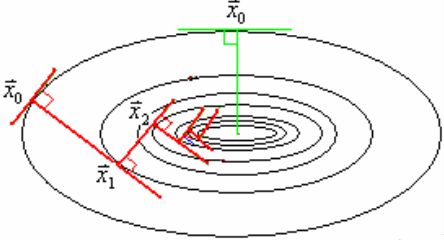
\includegraphics[width=.6\linewidth]{fig/zuisuxiajiangfa.png}
\end{center}

\subsection{Newton法}
\subsubsection{Newton法}

要求有二阶连续偏导数,且Hesse矩阵必须正定且显式。
记$f_k=f(\vec{x}_k),\vec{g}_k=\nabla f(\vec{x}_k),G_k=\nabla^2 f(\vec{x}_k)$。

对Taylor展开式的$f(\vec{x}^*)\approx f(\vec{x}_k)+g(\vec{x}_k)(\vec{x}^*-\vec{x}_k)+\frac{1}{2}(\vec{x}^*-\vec{x}_k)\Transpose G(\vec{x}_k) (\vec{x}^*-\vec{x}_k)$
观察右侧关于$\vec{x}^*$的二次函数,最小值取在$\vec{x}^*-\vec{x}_k = G(\vec{x}_k)^{-1} g(\vec{x}_k)$。
因此选择迭代选择$\vec{x}_{k+1} = \vec{x}_k - G(\vec{x}_k)^{-1}g(\vec{x}_k)$。

对正定二次函数,$G(\vec{x}_k)^{-1} g(\vec{x}_k) = Q^{-1} (Q \vec{x}_k + \vec{b})=\vec{x}_k + Q^{-1}\vec{b}$,
因此下一步直接收敛得到$\vec{x}_{k+1} = -Q^{-1}\vec{b}$。

Newton法的几何解释是使用二次曲面逼近局部,然后取二次曲面上的极小值点为下次的迭代点。

\begin{center}
    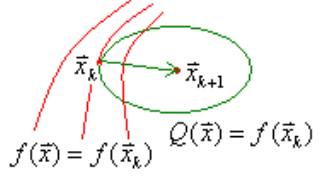
\includegraphics[width=.6\linewidth]{fig/niudunfa.png}
\end{center}

\subsubsection{修正Newton法*}

\subsection{共轭向量法与共轭梯度法}
\subsubsection{共轭向量}
关于从上次迭代点按二阶导数项拟合一个直接指向最小值的方向,得到$\vec{p}_0 Q\vec{p}_1=0$,因此做出以下定义:
\begin{definition}
    若$Q$是$n$阶正定矩阵,非零向量$\VectorComma{\vec{p}}{m}$满足$\vec{p}_i\Transpose Q\vec{p}_j=0$,
    称这组向量是$Q$共轭向量,或者这组向量是$Q$共轭的,这组向量对应的方向称为$Q$共轭方向。
\end{definition}

\begin{theorem}
    $Q$共轭的向量组线性无关。
\end{theorem}

\begin{definition}
    对线性无关向量组$\VectorComma{\vec{p}}{n}$,
    定义全体$\vec{z}=\vec{x}_0+\sum_i a_i\vec{p}_i$构成的集合为
    点$\vec{x}_0$与向量组$\VectorComma{\vec{p}}{n}$生成的线性流形,记为$L[\vec{x}_0;\VectorComma{\vec{p}}{n}]$。
\end{definition}

\subsubsection{共轭方向法}

\begin{theorem}
    给定$n$阶正定矩阵$Q$,$Q$共轭非零向量组$\vec{p}_0,\vec{p}_1,\dots,\vec{p}_{m-1}$,
    任意选取$\vec{x}_0$作为初始点进行$m$次直线搜索得到$\vec{x}_1,\dots,\vec{x}_{m}$,则有:
    $\vec{p}_j\Transpose \nabla f(\vec{x}_m) = 0$,
    且$\vec{x}_m$是二次函数$f(\vec{x})=\frac{1}{2}\vec{x}\Transpose Q \vec{x}+\vec{b}\Transpose\vec{x}+\vec{c}$极小点。
\end{theorem}

因为提供共轭方向的方法不同,共轭方向法有多种。

\subsubsection{共轭梯度法}

共轭梯度法是一种共轭向量法。

\begin{enumerate}
    \item 第一次迭代:
    \begin{enumerate}
        \item 搜索方向取$\vec{p}_0=-\vec{g}_0$;
        \item 步长$t_0=-\frac{\vec{p}_0\Transpose\vec{g}_0}{\vec{p}_0\Transpose Q \vec{p}_0}$;
        \item 迭代点$\vec{x}_1=\vec{x}_0+t_0\vec{p}_0$。
    \end{enumerate}
    \item 第二次迭代:
    \begin{enumerate}
        \item
        搜索方向:考虑和$\vec{p}_0$线性无关,设$\vec{p}_1=\vec{g}_1+\alpha_0 \vec{p}_0$,
        结合共轭条件$\vec{p}_0\Transpose Q \vec{p}_1=0$,
        可得$\alpha_0 = -\frac{\vec{g}_1\Transpose Q \vec{p}_0}{\vec{p}_0\Transpose Q\vec{p}_0}$,
        由此得到$\vec{p}_1$;
        \item 此时步长$t_1 = -\frac{\vec{p}_1\Transpose \vec{g}_1}{\vec{p}_1\Transpose Q \vec{p}_1 }$;
        \item 第二个迭代点$\vec{x}_2=\vec{x}_1+t_1\vec{p}_0$。
    \end{enumerate}
    \item 第$k$次($k>3$):
    \begin{enumerate}
        \item
        搜索方向:考虑和上次的$\vec{p}_{k-1}$线性无关,设$\vec{p}_k=\vec{g}_k+\alpha_{k-1} \vec{p}_{k-1}$,
        结合共轭条件$\vec{p}_k\Transpose Q \vec{p}_{k-1}=0$,
        可得$\alpha_{k-1} = -\frac{\vec{g}_k\Transpose Q \vec{p}_0}{\vec{p}_0\Transpose Q\vec{p}_0}$,
        由此得到$\vec{p}_k$;
        \item 此时步长$t_k = -\frac{\vec{p}_k\Transpose \vec{g}_k}{\vec{p}_k\Transpose Q \vec{p}_k }$;
        \item 第二个迭代点$\vec{x}_k = \vec{x}_{k-1}+t_1\vec{p}_k$。
    \end{enumerate}
\end{enumerate}

\paragraph{不使用Hesse矩阵的共轭梯度法*}

\subsection{拟Newton法}

考虑使用其他矩阵$H$近似Newton法中的$G^{-1}$。
每次使用$\vec{x}_{k+1}=\vec{x}_k - t_k H_k \vec{g}_k$迭代。
然后考查使$H$确实近似$G^{-1}$的条件:
\begin{itemize}
    \item $H_k$正定,以保证每次的搜索方向都是下降方向。
    \item 易于计算的迭代关系,迭代$H_k$的公式称为校正公式。
    \item 逆Newton条件:$\vec{x}_{k+1}-\vec{x}_k\approx H_{k+1} (\vec{g}_{k+1} - \vec{g}_k)$
\end{itemize}

\begin{itemize}
    \item DFP:选择$H_{k+1}=H_k + \alpha_k \vec{u}_k \vec{u}_k\Transpose + \beta_k \vec{v}_k \vec{v}_k\Transpose$
    作为校正公式,其中$\alpha_k,\beta_k,\vec{u}_k,\vec{v}_k$都是待定值。
    \item BFGS(*)
    \item Broyden算法族(*)
\end{itemize}

\subsection{步长加速法*}

\section{约束最优化方法}

最常见的是容许方向法和罚函数法。

\subsection{最优性条件}

\subsubsection{等式约束}
对含有等式约束的最优化问题,
\[
    \begin{array}{ll}
        \min & f(\vec{x})\\
        \SubjectTo & \vec{h}(\vec{x})=0 \\
    \end{array}
\]
令$L=f(\vec{x}) - \sum_i \lambda_i h_i(\vec{x})$,
极值点问题转化为求Lagrange函数的极值点,即
\[
    \nabla L =
    \begin{bmatrix}
        \nabla_{\vec{x}} L \\ \nabla_{\vec{\lambda}} L
    \end{bmatrix} =
    \begin{bmatrix}
        \nabla f(\vec{x}) + \sum\limits_i \lambda_i \nabla h_i(\vec{x}) \\
        h_1(\vec{x}) \\
        \vdots \\
        h_m(\vec{x})
    \end{bmatrix} = \vec{0}
\]
这一方法称为Lagrange乘子法。

\subsubsection{不等式约束的几何最优性条件}
\begin{definition}
    对容许集中一点,去到等号的不等式称为\textkw{起作用约束},否则称为\textkw{不起作用约束}。
    对内点,每个约束都是不起作用约束,对边界点,有至少一个起作用约束。
\end{definition}

\begin{definition}
    对从一点$\vec{x}$和方向向量$\vec{p}$,
    若$\exists \delta>0$使得$\forall t\in (0,\delta),\vec{x}+t\vec{p}\in D$,
    称为\textkw{容许方向}。
\end{definition}

\begin{definition}[锥。凸锥。]
\end{definition}

\begin{definition}
    全体容许方向向量构成\textkw{容许方向锥}。
    全体下降方向向量构成\textkw{下降方向锥}。
\end{definition}

\begin{theorem}[几何最优性条件]
    下降方向锥与容许方向锥交集为空。
\end{theorem}
这是一个必要条件。

\subsubsection{F-J条件}
\begin{lemma}[Farkas引理]
    对$n$维向量$\VectorComma{a}{m},b$,有:
    $a_i\Transpose p>0,i=1,2,\dots,m\Rightarrow b\Transpose p>0\Leftrightarrow \exists \VectorComma{\gamma}{m}>0,b=\sum\limits_i \gamma_i a_i$。
\end{lemma}

\begin{lemma}[Gordan引理]
    对$n$维向量$\VectorComma{a}{m}$,有:
    $\nexists p,\vec{a}\Transpose p<0,i=1,2,\dots,m \Rightarrow \exists \VectorComma{\gamma}{m}\geq 0,b=\sum\limits_i \gamma_i a_i=\vec{0}$。
\end{lemma}

\begin{theorem}[Fritz-John条件]
    $\vec{x}^*$是极小点$\Rightarrow\exists \mu_0,\linebreak[1]\mu_1,\linebreak[1]\dots,\linebreak[1]\mu_m\text{不全为零}$,使得:
    \[
        \begin{cases}
            \mu_0\nabla f(\vec{x}^*) - \sum\limits_i\mu_i\nabla s_i(\vec{x}^*) = 0 &\quad\text{(Lagrange函数)} \\
            \mu_i s_i(\vec{x}^*) = 0, i=1,2,\dots,m & \quad\text{(互补松弛条件)} \\
            \mu_i \geq 0, i=1,2,\dots,m & \\
        \end{cases}
    \]
    这个必要条件称为F-J条件,满足F-J条件的所有点称为F-J点。
    式中的$\mu_0,\mu_1,\dots,\mu_m$称为Lagrange乘子。
\end{theorem}

\subsubsection{K-T条件}
约束F-J条件的$\mu_0=1$得到K-T条件。
\begin{theorem}[Kuhn-Tucker条件]
    $\vec{x}^*$是极小点$\Rightarrow\exists \mu_1,\linebreak[1]\dots,\linebreak[1]\mu_m$,使得:
    \[
        \begin{cases}
            \mu_0\nabla f(\vec{x}^*) = \sum\limits_i\mu_i\nabla s_i(\vec{x}^*) &\quad\text{(Lagrange函数)} \\
            \mu_i s_i(\vec{x}^*) = 0, i=1,2,\dots,m & \quad\text{(互补松弛条件)} \\
            \mu_i \geq 0, i=1,2,\dots,m & \\
        \end{cases}
    \]
    这个必要条件称为K-T条件或KKT条件(KKT指Karush-Kuhn-Tucker),满足K-T条件的所有点称为K-T点。
\end{theorem}

\begin{theorem}
    起作用的$\nabla s$线性无关,且$\mu_0\neq 0$的F-J点必为K-T点。
\end{theorem}

\begin{theorem}
    对凸规划,其中$f$可微凸函数,$s$可微凹函数,$h$线性函数,则K-T点都是全局最优点。
\end{theorem}

\subsection{外部罚函数法}
对最优化问题,定义增广目标函数
\[
    \begin{split}
        F(\vec{x},\mu) &= f(\vec{x}) + \mu \alpha(\vec{x}) \\
        \alpha(\vec{x}) &= \sum_j [h_j (\vec{x})]^2 + \sum_i [s_i(\vec{x})]^2 u(s_i(\vec{x})) \\
    \end{split}
\]
$F$称为增广目标函数,
$\mu$为罚因子,第二项$\mu\alpha(\vec{x})$称为惩罚项,
其中的$u(t)$是一个阶跃函数,定义为
\[
    u(t)=\begin{cases}0,t \geq 0\\1,t<0\end{cases}
\]

\begin{theorem}
    给定$\mu$,若$\vec{x}_\mu$是无约束问题$\min F(\vec{x},\mu)$的极小点,
    则$\vec{x}_\mu$是有约束问题$\min f(\vec{x}) \SubjectTo h_j(\vec{x})=0, s_i(\vec{x})\geq 0$的极小点的
    充要条件是$\vec{x}_\mu$是有约束问题的容许点。
\end{theorem}

对于一般的$\vec{x}\notin C$,需要增大$\mu$计算,
一般认为$\mu=1,2,\dots$得到序列$\{\vec{x}_k\}$,
则若$\{\vec{x}_k\}$收敛,一定能收敛在极小点。
这种方法称为\textkw{外部罚函数法}或\textkw{外点法}。
这种通过解无约束问题进而解决有约束问题的方法,也称为``序列无约束最小化技术''(SUMT)。

\subsection{内部罚函数法}
外点法取在外部并逐渐向容许集边界移动,因此其可能难以取到容许集内的点,
或者可能函数在容许集外根本无法定义,导致不能用外点法计算出极小点。
为保证迭代点总是内点,则产生了内部罚函数法。

初始点$\vec{x}_0$选择内点,然后设计障碍函数
\[
    \begin{split}
        F(\vec{x},\mu) &= f(\vec{x}) + \mu\beta(\vec{x}) \\
        \beta(\vec{x}) &= \sum_i \frac{1}{s_i(\vec{x})} \\
    \end{split}
\]
$F$为障碍函数,
$\mu$为罚因子,第二项$\mu\beta(\vec{x})$为惩罚项。
$\beta$也可以取如$\sum\ln \frac{1}{s(\vec{x})}, \sum \frac{1}{s^2(\vec{x})}, \sum\frac{1}{s(\vec{x}) u[-s(\vec{x})]}$等的函数。

选择一个内点作为初始点,通过$\mu\to 0^+$,得到极小点。

注意内部罚函数法有无法处理等式约束的严重缺陷,
产生的结合两种罚函数法的优势得到了混合罚函数法。

\subsection{乘子法}
外部罚函数法中,随着罚因子增大,Hesse矩阵条件数增大,数值计算的稳定性变差导致计算结果不精确,
于是产生了乘子法。

\paragraph{H乘子法*}
\paragraph{R乘子法*}

\subsection{Zoutendijk容许方向法*}

\section{多目标规划}
同时对多个目标进行优化即多目标规划问题。

\subsection{数学模型}
不等式约束转换为大于等于后,可得数学模型:
\[
    \begin{array}{ll}
        \min & f_1(\VectorComma{x}{n}) \\
        \min & f_2(\VectorComma{x}{n}) \\
        & \dots \\
        \min & f_p(\VectorComma{x}{n}) \\
        \max & g_1(\VectorComma{x}{n}) \\
        \max & g_2(\VectorComma{x}{n}) \\
        & \dots \\
        \max & g_q(\VectorComma{x}{n}) \\
        \SubjectTo & s_i(\VectorComma{x}{n})\geq 0 \\
        & h_j(\VectorComma{x}{n}) = 0 \\
    \end{array}
\]
将最大转换为最小,写成向量形式,记
\[
    \begin{split}
        \vec{x} &= (\VectorComma{x}{n})\Transpose \\
        \vec{f}(\vec{x}) & =(f_1(\vec{x}),f_2(\vec{x}),\dots,f_p(\vec{x}),f_{p+1}(\vec{x}),\dots,f_r(\vec{x}))\Transpose \\
        f_{p+k}(\vec{x}) & = -g_{k}(\vec{x}) \\
        D &= \{\vec{x}\mid s_i(\vec{x})\geq 0,h_i(\vec{x}) = \vec{0}\} \\
    \end{split}
\]
则原问题可记为
\[
    \mathbf{v-}\min_{\vec{x}\in D} \vec{f}(\vec{x})
\]
称为向量极小化模型,$\vec{f}(\vec{x})$称为向量目标函数,其分量称为分量目标函数。

对各分量目标函数为线性的情况,可通过线性替换使得$\vec{s}(\vec{x})$转化为
\[
    \begin{array}{rl}
        \mathbf{v-}\min\limits_{\vec{x}} & \vec{f}(\vec{x}) = C\vec{x} \\
        \SubjectTo & A\vec{x} = \vec{b} \\
        & \vec{x} \geq \vec{0} \\
    \end{array}
\]

\subsection{解的概念与性质}
\begin{definition}[向量的序关系]
    \begin{gather*}
        \vec{a} < \vec{b} \Leftrightarrow \vec{b} > \vec{a} \Leftrightarrow \forall i,a_i<b_i \\
        \vec{a} \leq \vec{b} \Leftrightarrow \vec{b} \geq \vec{a} \Leftrightarrow \forall i,a_i\leq b_i \\
        \vec{a} \prec \vec{b} \Leftrightarrow \vec{b} \succ \vec{a} \Leftrightarrow \forall i, a_i\leq b_i \land \exists i, a_i\neq b_i\\
    \end{gather*}
\end{definition}

\begin{definition}[不同程度的最优解]
    为确定``好''解,定义:
    \begin{itemize}
        \item
        对$\vec{f}(\vec{x})$,给定$\vec{x}^*$,
        若$\forall \vec{x} \in D, \vec{f}(\vec{x}) \geq \vec{f}(\vec{x}^*)$,
        则称$\vec{x}^*$为\textkw{绝对最优解}。
        全体绝对最优解的集合为\textkw{绝对最优解集},记作$X^*(\vec{f},D)$。
        \item
        对$\vec{f}(\vec{x})$,给定$\vec{x}^*$,
        若$\nexists \vec{x} \in D, \vec{f}(\vec{x}) \prec \vec{f}(\vec{x}^*)$,
        则称$\vec{x}^*$为\textkw{有效解}或\textkw{Pareto解}。
        全体有效解的集合为\textkw{有效解集},记作$P(\vec{f},D)$。
        \item
        对$\vec{f}(\vec{x})$,给定$\vec{x}^*$,
        若$\nexists \vec{x} \in D, \vec{f}(\vec{x}) < \vec{f}(\vec{x}^*)$,
        则称$\vec{x}^*$为\textkw{弱有效解}。
        全体弱有效解的集合为\textkw{弱有效解集},记作$P_w(\vec{f},D)$。
    \end{itemize}
\end{definition}

\begin{theorem}
    $X^* \subseteq P \subseteq P_w \subseteq D$,
    且$X^*=\bigcap\limits_i X^*_i,\bigcup\limits_i X^*_i\subseteq P_w$。
    其中$X^*,P,P_w$分别为绝对最优、有效、弱有效解,
    $X^*_i$为第$i$个分量目标函数的最优解集。
\end{theorem}

\begin{theorem}
    若$X^*\neq \emptyset$,则$P=X^*$。
    若$D$是凸集,每个分量目标函数$f_i$是凸函数,则$P=P_w$。
\end{theorem}

\subsection{评价函数法}
\begin{definition}[多元函数单调性]
    多元函数$\varphi:\mathbb{R}^r\to\mathbb{R}$:
    若$\forall \vec{z}_1<\vec{z}_2,\varphi(\vec{z}_1)<\varphi(\vec{z}_2)$,称$\varphi(\vec{z})$单调增函数;
    若$\forall \vec{z}_1\prec\vec{z}_2,\varphi(\vec{z}_1)<\varphi(\vec{z}_2)$,称$\varphi(\vec{z})$严格单调增函数。
\end{definition}

\begin{theorem}
    对多目标规划$\vec{f}(\vec{x})$,
    考虑$\min\limits_{x\in D} \varphi(\vec{f}(\vec{x}))$有极小点$\vec{x}^*$,则:
    \begin{itemize}
        \item 若$\varphi$是严格增函数,$x^*\in P(\vec{f}, D)$
        \item 若$\varphi$是增函数,$x^* \in P_w(\vec{f}, D)$
    \end{itemize}
\end{theorem}
称这样的$\varphi$为评价函数。

\subsubsection{常见评价函数}

\paragraph{线性加权和}
取评价函数$\varphi(\vec{z})=\vec{u}\vec{z},u_i\geq 0,\sum u_i=1$为\textkw{线性加权和函数},
其中$\vec{u}$为\textkw{权向量},且:
$\vec{u}>0$时,严格单调增;$\vec{u}\succ \vec{0}$时,单调增。
这样的方法称为\textkw{线性加权和法}。

\paragraph{理想点函数}
取评价函数$\varphi(\vec{z})=\|\vec{z}-\vec{z}^*\|$为\textkw{理想点函数},
其中$\vec{z}^*$是每个分量函数能取到的最小值,称为\textkw{理想点},
这样的方法称为\textkw{理想点法}。

\paragraph{平方加权函数}
考虑理想点函数中范数进行平方,取加权的二次方和的情况,
取评价函数$\varphi(\vec{z})=\sum\limits_i (\vec{z}_i-\vec{z}_i^*)$。
这样的方法称为\textkw{平方加权和法}。

\paragraph{极大函数}
取评价函数$\varphi(\vec{z})=\max\{z_i\}$或加权的$\max\{u_i z_i\}$,
这样的方法称为\textkw{极大极小法}。
由于直接求这个极大值的极小值较难,通常转化为$\min v \SubjectTo u_i f_i(\vec{x})\leq v,x\in D$来求解,
其中$v$称为松弛变量。

\subsubsection{权重的确定}
\paragraph{去量纲处理}
首先需要将各不同目标函数的量纲去除。

\paragraph{老手法}
选择多位相关专家和有实践经验的工作者,统计其对不同项目的权重的估计值,然后求取平均。
求平均后需要检查每个人与平均结果的最大偏差,若偏差足够小则认为大家的经验无差别,可以使用,
否则需要再次进行协商调整并重复此流程。

\paragraph{$\alpha$法}
借助各分量目标函数在容许集上的极小值点确定权重的方法。
通过最小化不同的分量目标函数得到极小值点$\VectorComma{\vec{x}^*}{r}$,
在自变量取这些值时得到向量目标函数的取值$\vec{z}^*_i=\vec{f}(\vec{x}^*_i)$。
若这是$r$个不同的点,撑起一个$r$维空间中的超平面,
设$\vec{u}\Transpose \vec{z}=\alpha$,
改变合适的$\alpha$值使得$\vec{u}$每个分量非负且和为$1$,
则得到一个可用的权重向量$\vec{u}$。

\section{标量的矩阵求导术}
\begin{definition}
    对矩阵函数$f:F^{m\times n}\to F$,定义对矩阵的导数
    $\frac{\partial f}{\partial A}=\left(\frac{\partial f}{\partial a_{ij}}\right)_{m\times n}$
\end{definition}

\begin{itemize}
    \item $f(A)=X\Transpose AY,\frac{\partial f}{\partial A}=XY\Transpose$
    \item $f(A)=\TraceOf(AB)=\TraceOf(BA),\frac{\partial f}{\partial A} = B\Transpose$
    \item $f(A)=\TraceOf(A\Transpose C)=\TraceOf(CA\Transpose)=A\bullet C,\frac{\partial f}{\partial A}=C$
    \item $f(A)=\TraceOf(A\Transpose A)=\TraceOf(AA\Transpose)=\|A\|_F^2,\frac{\partial f}{\partial A}=2A$
    \item $f(A)=\TraceOf(A\Transpose AB),\frac{\partial f}{\partial A}=AB+AB\Transpose$
    \item $f(A)=\TraceOf(A\Transpose BA),\frac{\partial f}{\partial A}=BA+B\Transpose A$
    \item $f(A)=\TraceOf(PAQ)=\TraceOf(AQP),\frac{\partial f}{\partial A}=P\Transpose Q\Transpose$
\end{itemize}

\end{document}
